\chapter{SCI-HI System Development}\label{Ch:System}



\section{Overview} \label{Sec:sysover}

$''$Sonda Cosmologica de las Islas para la Deteccion de Hidrogeno Neutro$''$ (SCI-HI) is an experiment which seeks to measure the \cm global spectrum during the end of the Dark Ages and the Cosmic Dawn before reionization. SCI-HI is a collaboration between Carnegie Mellon University (CMU) and Instituto Nacional de Astrof\'{i}sica, \'{O}ptica y Electr\'{o}nica (INAOE) in Mexico.  

The SCI-HI instrument was designed to meet several distinct contraints:

\begin{enumerate}
\item The instrument must be low cost (under \$10,000).

\item The instrument must be low power (under  200 Watts) so that it can be run with an independent power source separate from external supplies. 

\item The instrument must be simple and easy to deploy to remote locations. 

\item The instrument must be broadband to cover the wide bandwidth of interest ($40-130 MHz$).

\item The instrument must include a system response that varies smoothly with frequency. 

\end{enumerate}

\begin{figure}[bht]
\begin{center}
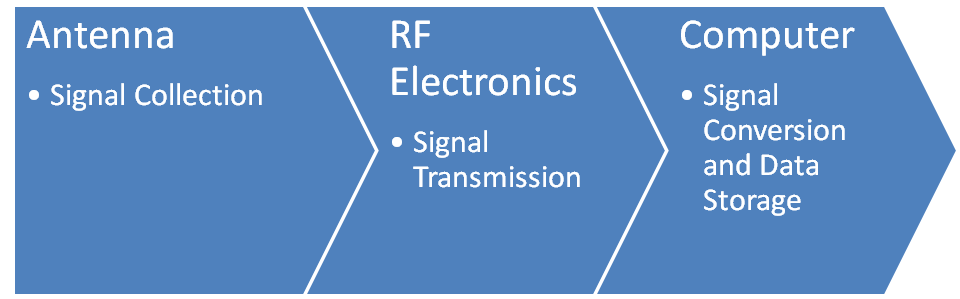
\includegraphics[width=0.9\linewidth]{SCIHI_system/figures/basic_block_diagram.png}
\caption{High level block diagram of the SCI-HI instrument with the three primary sections of the experiment. }
\label{Fig:basic_block_diagram}
\end{center}
\end{figure}

In order to meet these constraints, the instrument design was broken down into three sections based upon their purpose in the overall design (see Figure \ref{Fig:basic_block_diagram}). These sections are: (a) an antenna for signal collection, (b) radio frequency (RF) electronics for calibration and signal transmission, and (c) a computer to sample the signal, then process and store its spectrum. 



\section{Antenna}


\subsection{Antenna Design Constraints}

The SCI-HI experiment needs a single dipole antenna that meets four design constraints. 

\begin{enumerate}

\item The antenna radiation (beam) pattern must be stable over a wide bandwidth. 

\item The antenna beam must have a main lobe centered at zenith and small side-lobes. 

\item The antenna impedance must be stable and have a small reactance over its bandwidth. 

\item The antenna must be small enough for easy transport and set up in remote locations. 

\end{enumerate}

To identify an antenna that meets the first three constraints, we utilized two design strategies. First, we simulated the antenna design using commercially available software to identify a basic design that met our criteria. Second, we used an antenna chamber to measure the antenna's beam and impedance. 

\subsubsection{Antenna Beam Shape Measurement}

Measurement of an antenna's beam shape requires a special facility called an antenna range. The antenna range has a transmitting antenna with well known properties and an anechoic chamber large enough for the transmitting antenna and antenna-under-test to be in the far-field regime. Measurement is made by rotating the antenna-under-test with respect to the transmitting antenna. Meanwhile, the distance between the two antennas is held constant. The magnitude of the signal recieved by the antenna-under-test will change as a function of rotation angle. Mapping this magnitude over many angles gives the antenna's beam pattern. 

\subsubsection{Antenna Impedance Measurement} 

Antenna impedance is measured at an antenna range by connecting a Vector Network Analyzer to the antenna's terminal. A signal is sent down a cable from the analyzer into the antenna-under-test. The fraction of the original signal that is reflected back into the analyzer is measured. This reflection is called the reflectivity, or $S11$, and can be converted into impedance by comparing it to the reflection of a reference with known impedance. The conversion to impedance will be discussed in Section \ref{Sec:HIbiscus_Imp} \cite{stutzman1981}.

\begin{figure}[htb]
\centering
\begin{minipage}[b]{0.45\textwidth}
\centering
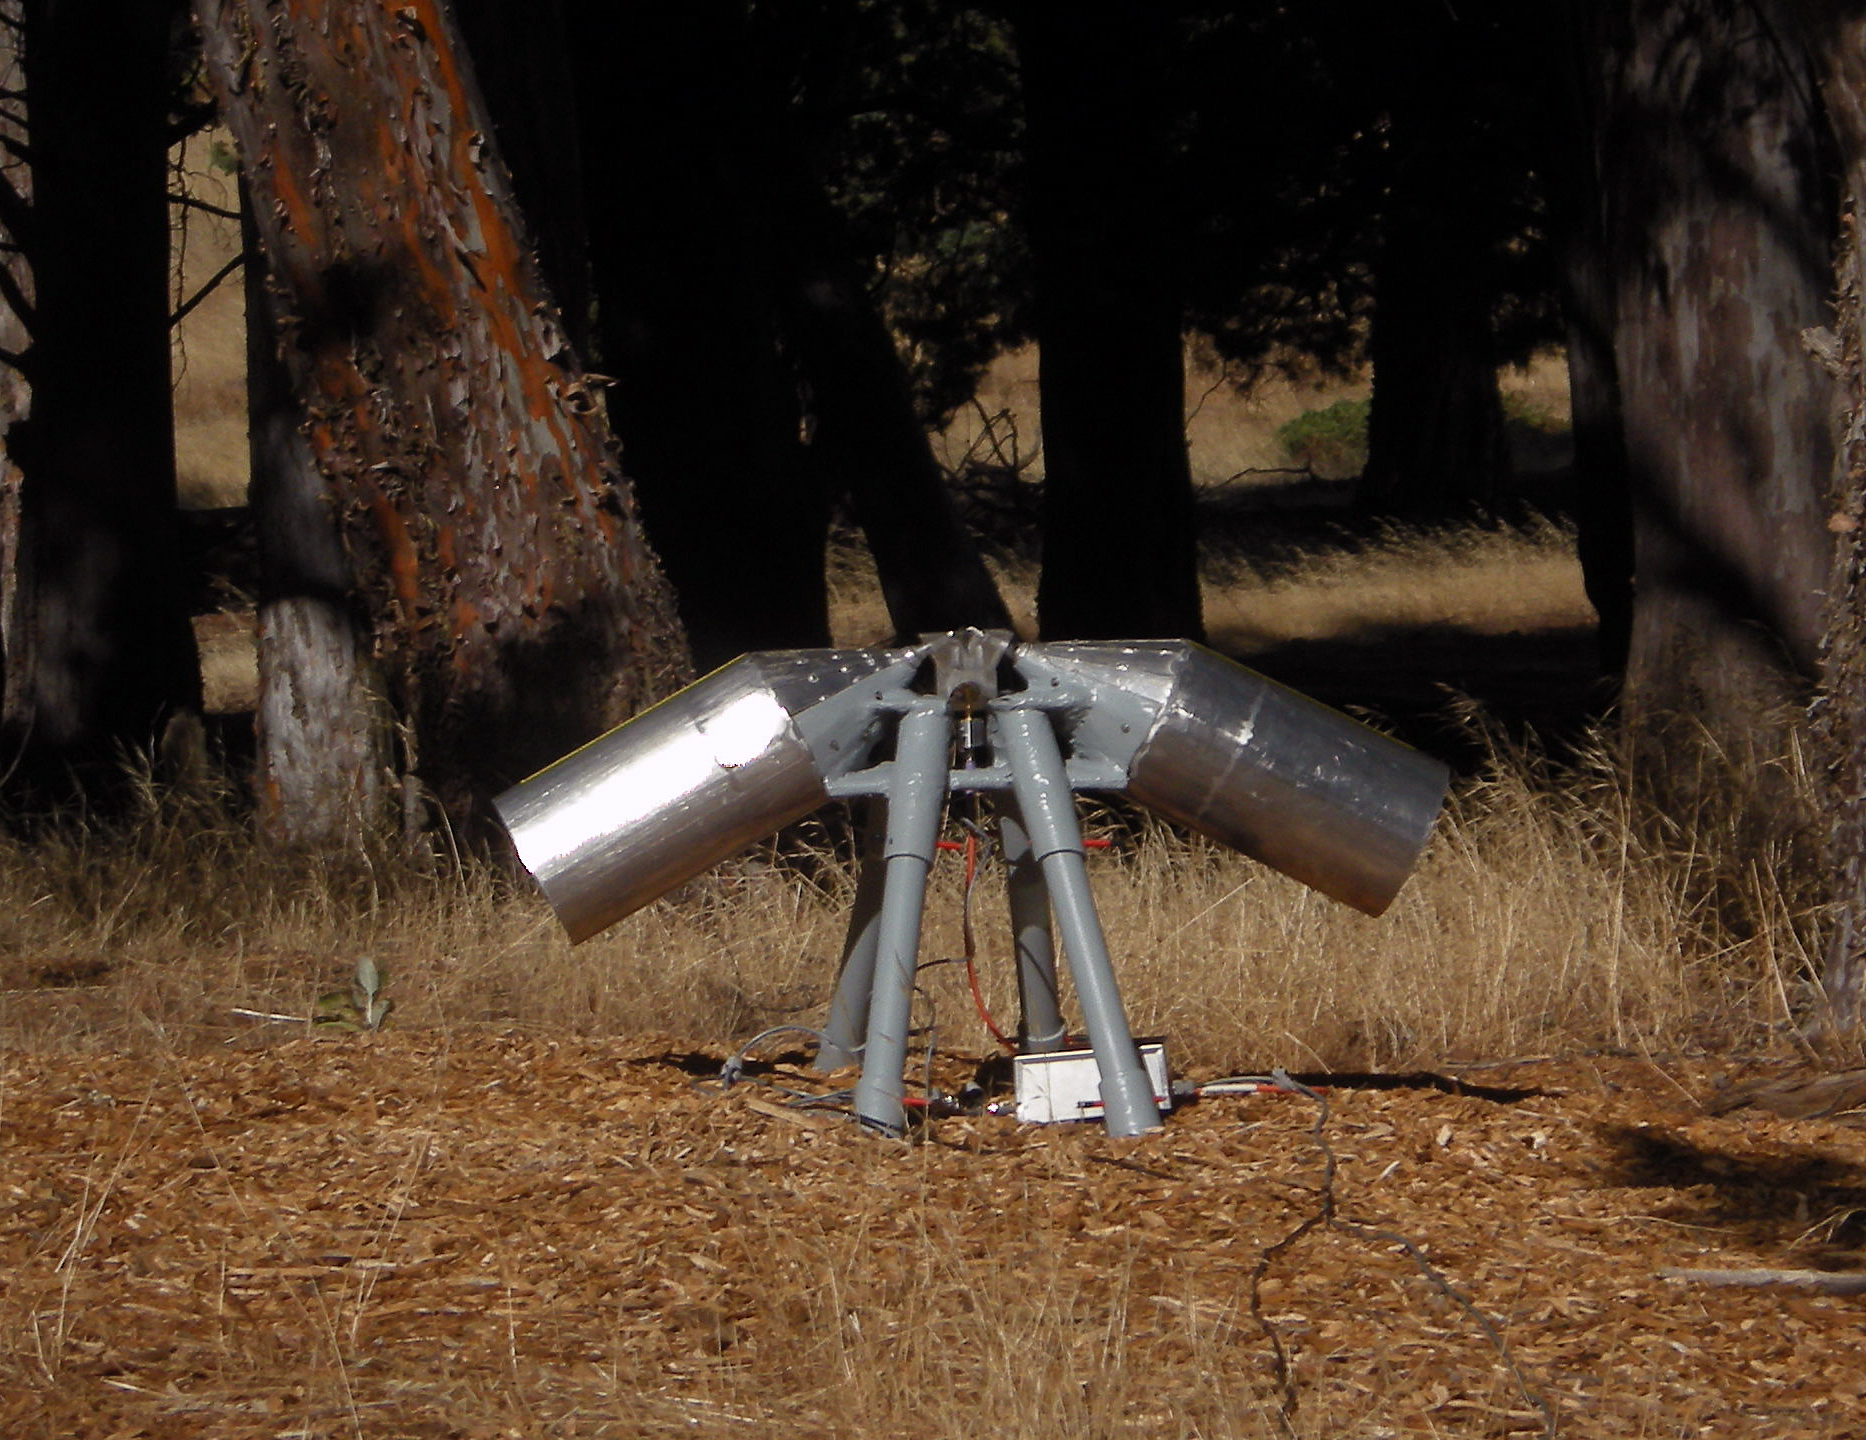
\includegraphics[width=0.95\linewidth]{SCIHI_system/figures/trombone_guad_small.jpg}
\caption{Trombone antenna set-up in its smallest (highest center frequency) configuration. }
\label{Fig:trombone_small}
\end{minipage}%
\begin{minipage}[b]{0.02\textwidth}
\hspace{1cm}
\end{minipage}%
\begin{minipage}[b]{0.51\textwidth}
\centering
\includegraphics[width=0.95\linewidth]{SCIHI_system/figures/trombone_pgh_zoom.jpg}
\caption{Trombone antenna set-up in its largest (lowest center frequency) configuration.}
\label{Fig:trombone_large}
\end{minipage}
\end{figure}


\subsection{Trombone Antenna}

For the first version of the SCI-HI antenna, we started with a simple $''$Trombone$''$ antenna. This design is based on the U.S. Naval Research Laboratory's Low-frequency Test Array (NLTA) dipole \cite{ellingson_2005}. The design is a dipole with fat, angled elements over a ground plane and is shown in Figures \ref{Fig:trombone_small} and \ref{Fig:trombone_large}. Changing the frequency range of the antenna (aka tuning) requires shifting the length of the dipole elements and their height above a ground plane. 

We selected the Trombone antenna for its tuning capabilities. Tuning of the antenna causes features in the measured spectrum from the antenna design to shift in frequency. On the other hand, features in the measured spectrum which are from the sky stay at the same frequencies when the antenna is tuned. Lack of shifting during tuning allows us to distinguish real structure on the sky such as the \cm signal from structure due to the antenna. 

\begin{figure}[htb]
\centering
\begin{minipage}[b]{0.53\textwidth}
\centering
\includegraphics[width=0.95\linewidth]{SCIHI_system/figures/trombone_mount.jpg}
\caption{Mounting for the Trombone antenna, with a lucite mount point and fiberglass support structure. }
\label{Fig:trombone_mount}
\end{minipage}%
\begin{minipage}[b]{0.02\textwidth}
\hspace{1cm}
\end{minipage}%
\begin{minipage}[b]{0.41\textwidth}
\centering
\includegraphics[width=0.95\linewidth]{SCIHI_system/figures/trombone_guad_adj.jpg}
\caption{Tabitha in the process of tuning the Trombone antenna between measurements.}
\label{Fig:trombone_adj}
\end{minipage}
\end{figure}

\subsubsection{Antenna Construction}

The original Trombone antenna used in the SCI-HI experiments was constructed by Edgar Castillo, a graduate student visiting CMU from INAOE in 2011. The trombone shapes were constructed out of welded aluminum with a lucite mounting block at the connection point of the two cones (see Figure \ref{Fig:trombone_mount}), The dipoles and mounting block were supported with a structure constructed out of fiberglass and PVC pipes. The entire system was placed above a ground plane composed of two parts: (a) metal mesh (aka chicken wire) with a small $\sim9 m^2$ area and (b) long radial extensions ($\sim10 m$) extending out from the center like a spider web. Tuning the Trombone antenna length was done by adding an external alumnium tube that slid over the main dipole elements (see Figure \ref{Fig:trombone_adj}). Meanwhile, tuning the height of the Trombone antenna was done using extendable PVC pipe support legs.

\begin{figure}[htb]
\centering
\begin{minipage}[b]{0.48\textwidth}
\centering
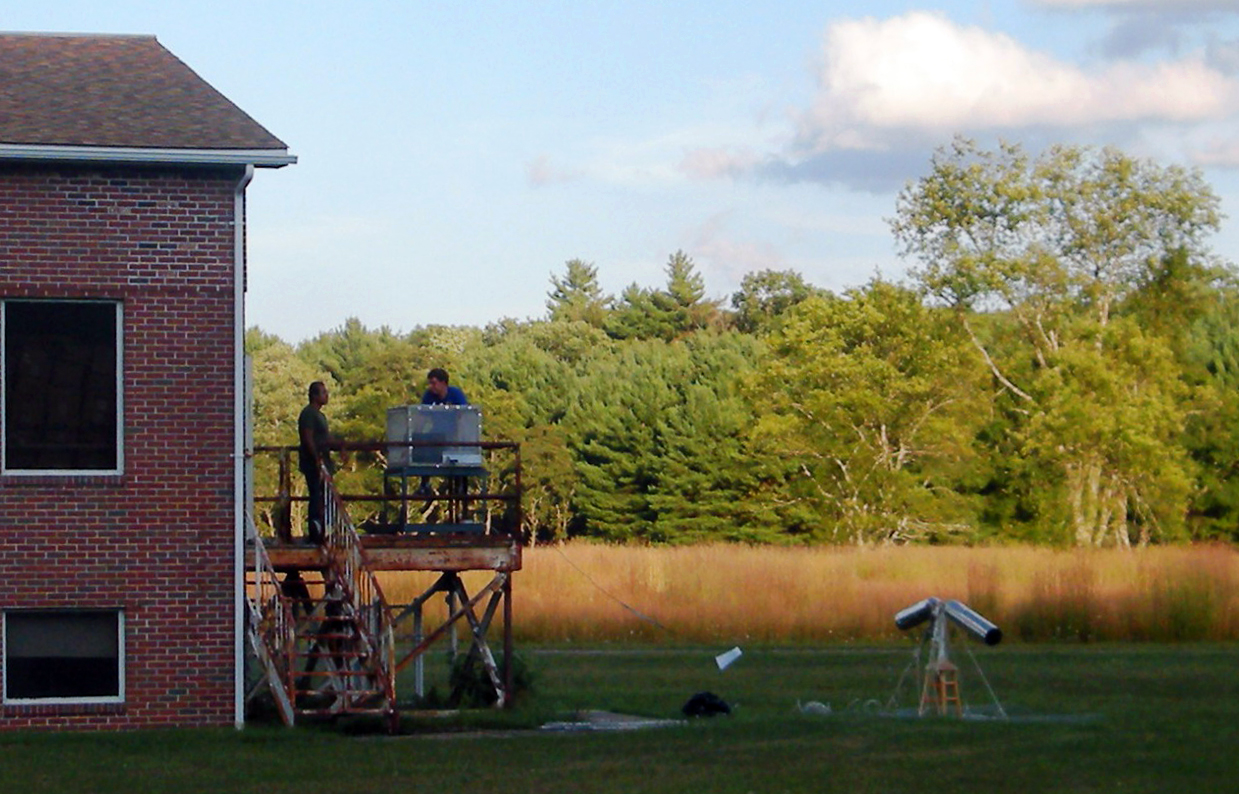
\includegraphics[width=0.95\linewidth]{SCIHI_system/figures/trombone_gbt.jpg}
\caption{SCI-HI setup with Trombone antenna on site at Green Bank in August 2011.}
\label{Fig:trombone_gbt}
\end{minipage}%
\begin{minipage}[b]{0.02\textwidth}
\hspace{1cm}
\end{minipage}%
\begin{minipage}[b]{0.46\textwidth}
\centering
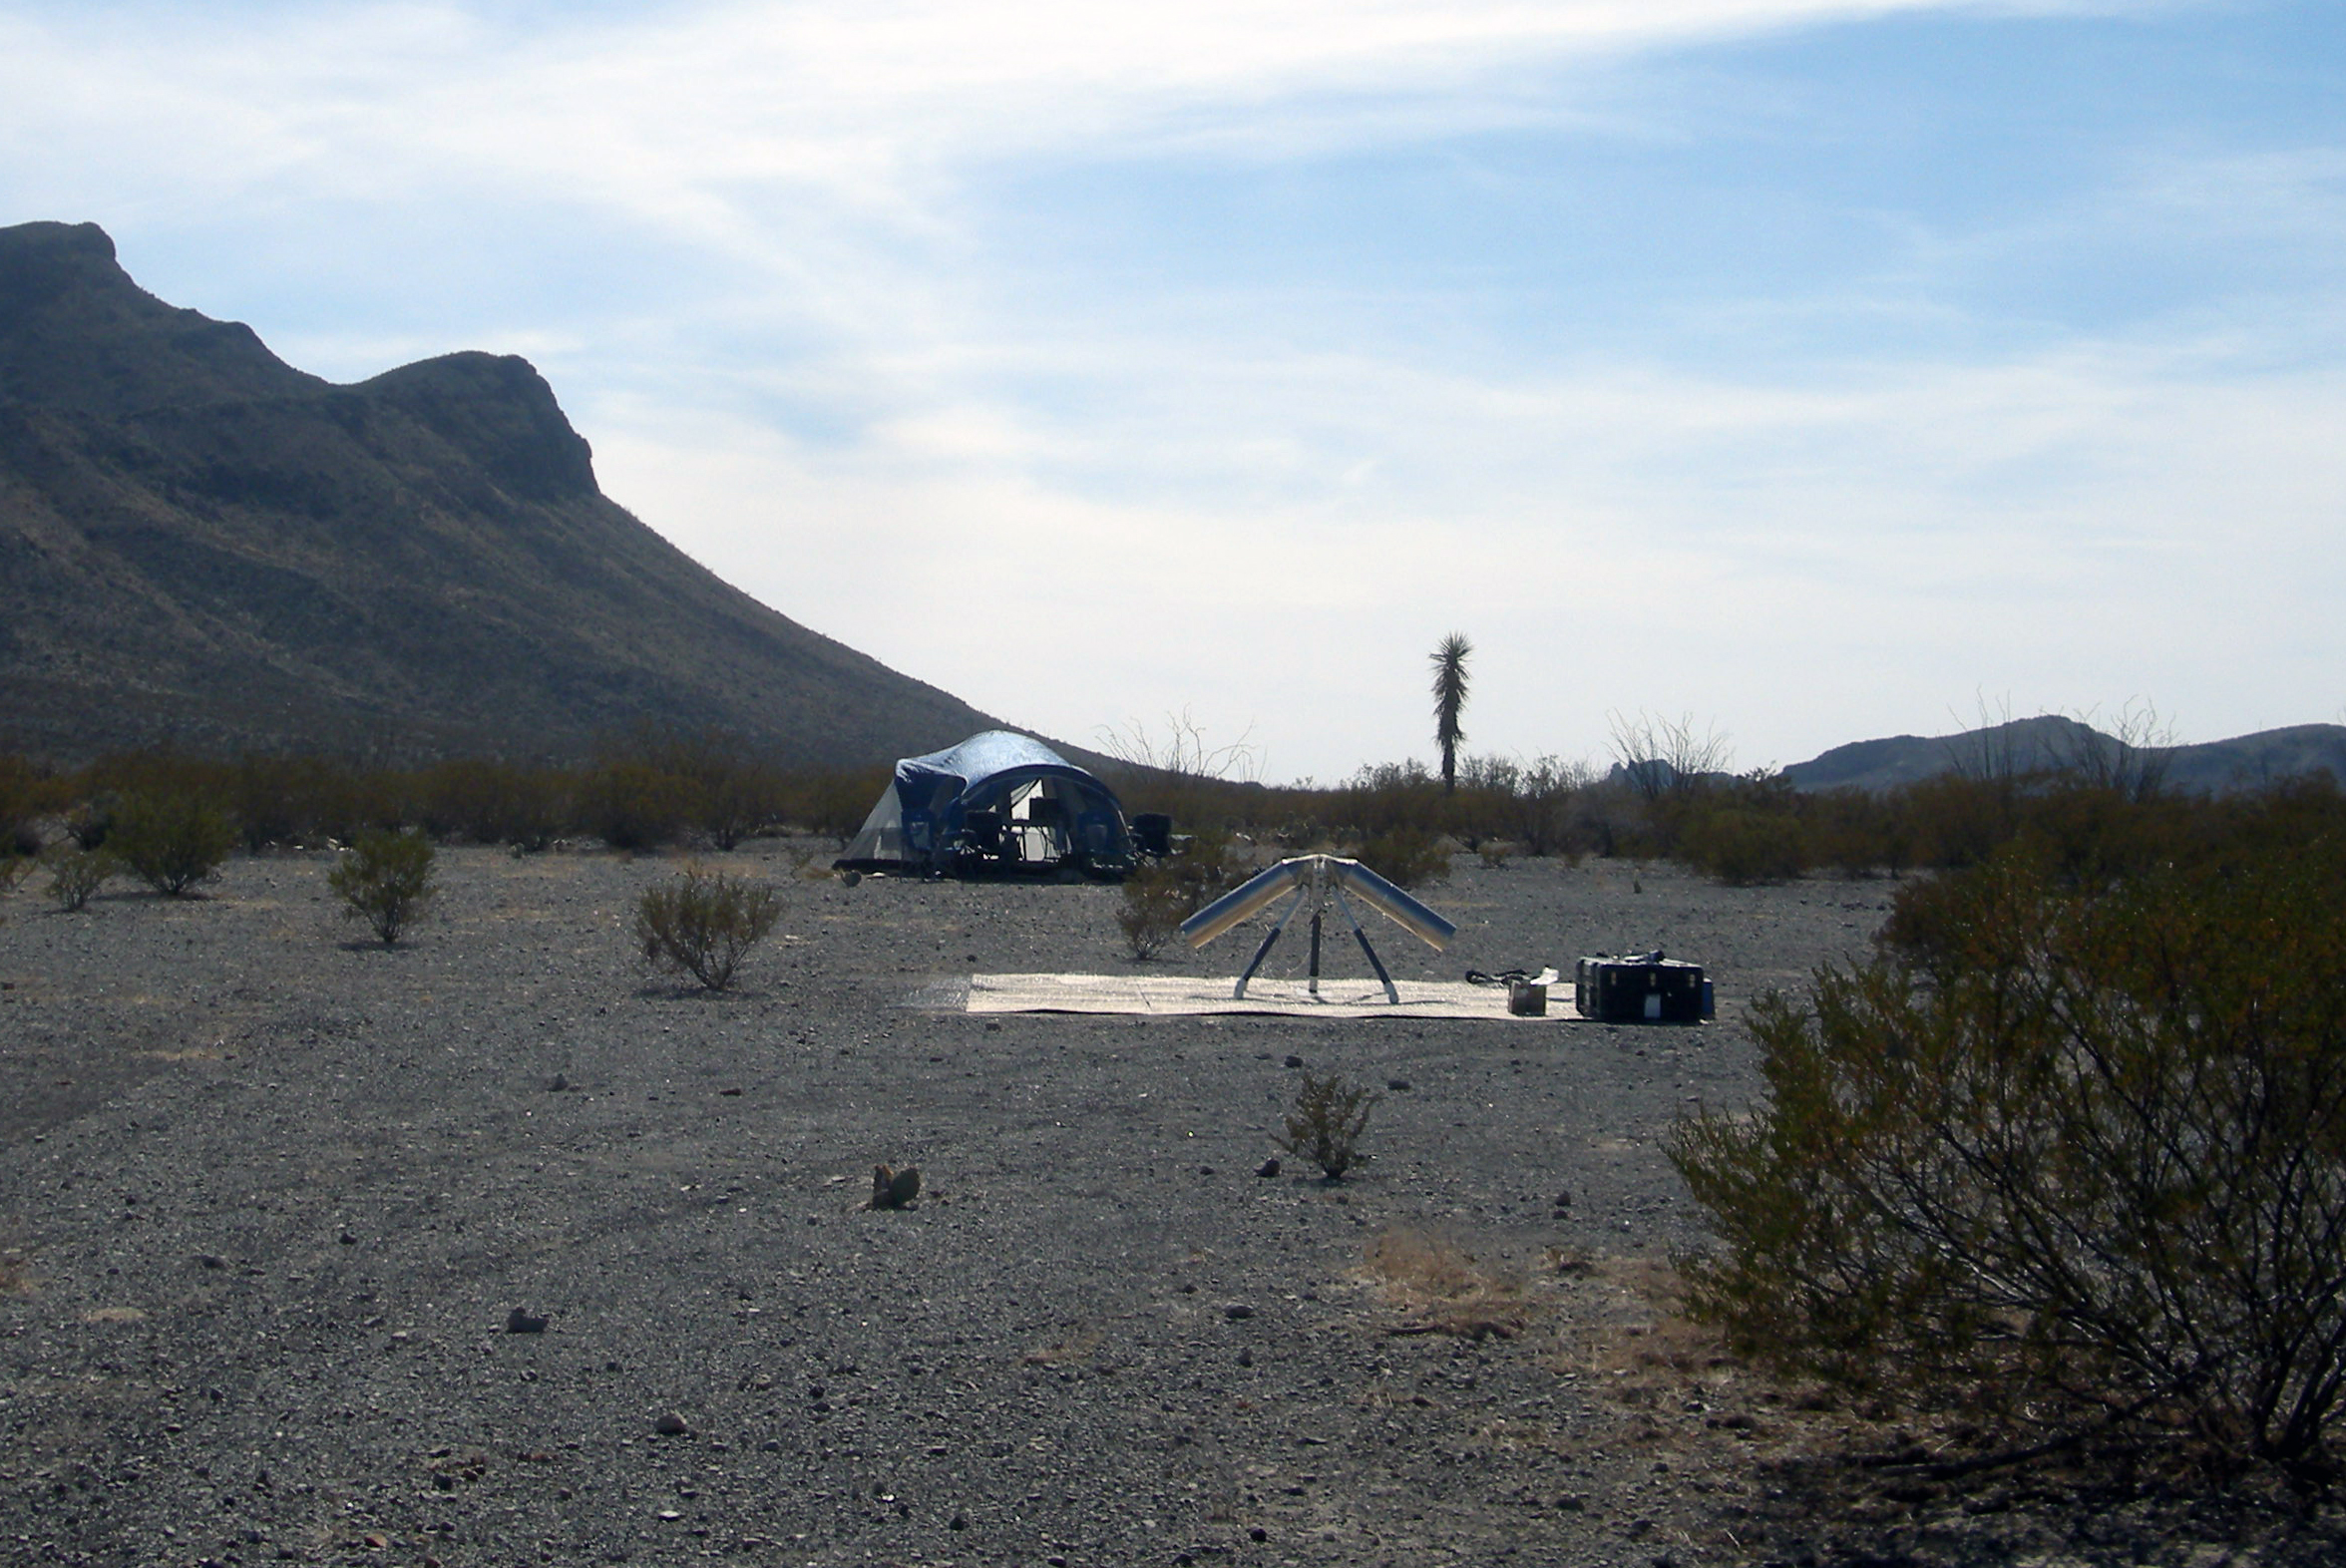
\includegraphics[width=0.95\linewidth]{SCIHI_system/figures/trombone_sys_ZdS.jpg}
\caption{SCI-HI setup with Trombone antenna on site at the Zona del Silencio in January 2012.}
\label{Fig:trombone_zds}
\end{minipage}
\end{figure}

\begin{figure}[htb]
\centering
\begin{minipage}[b]{0.52\textwidth}
\centering
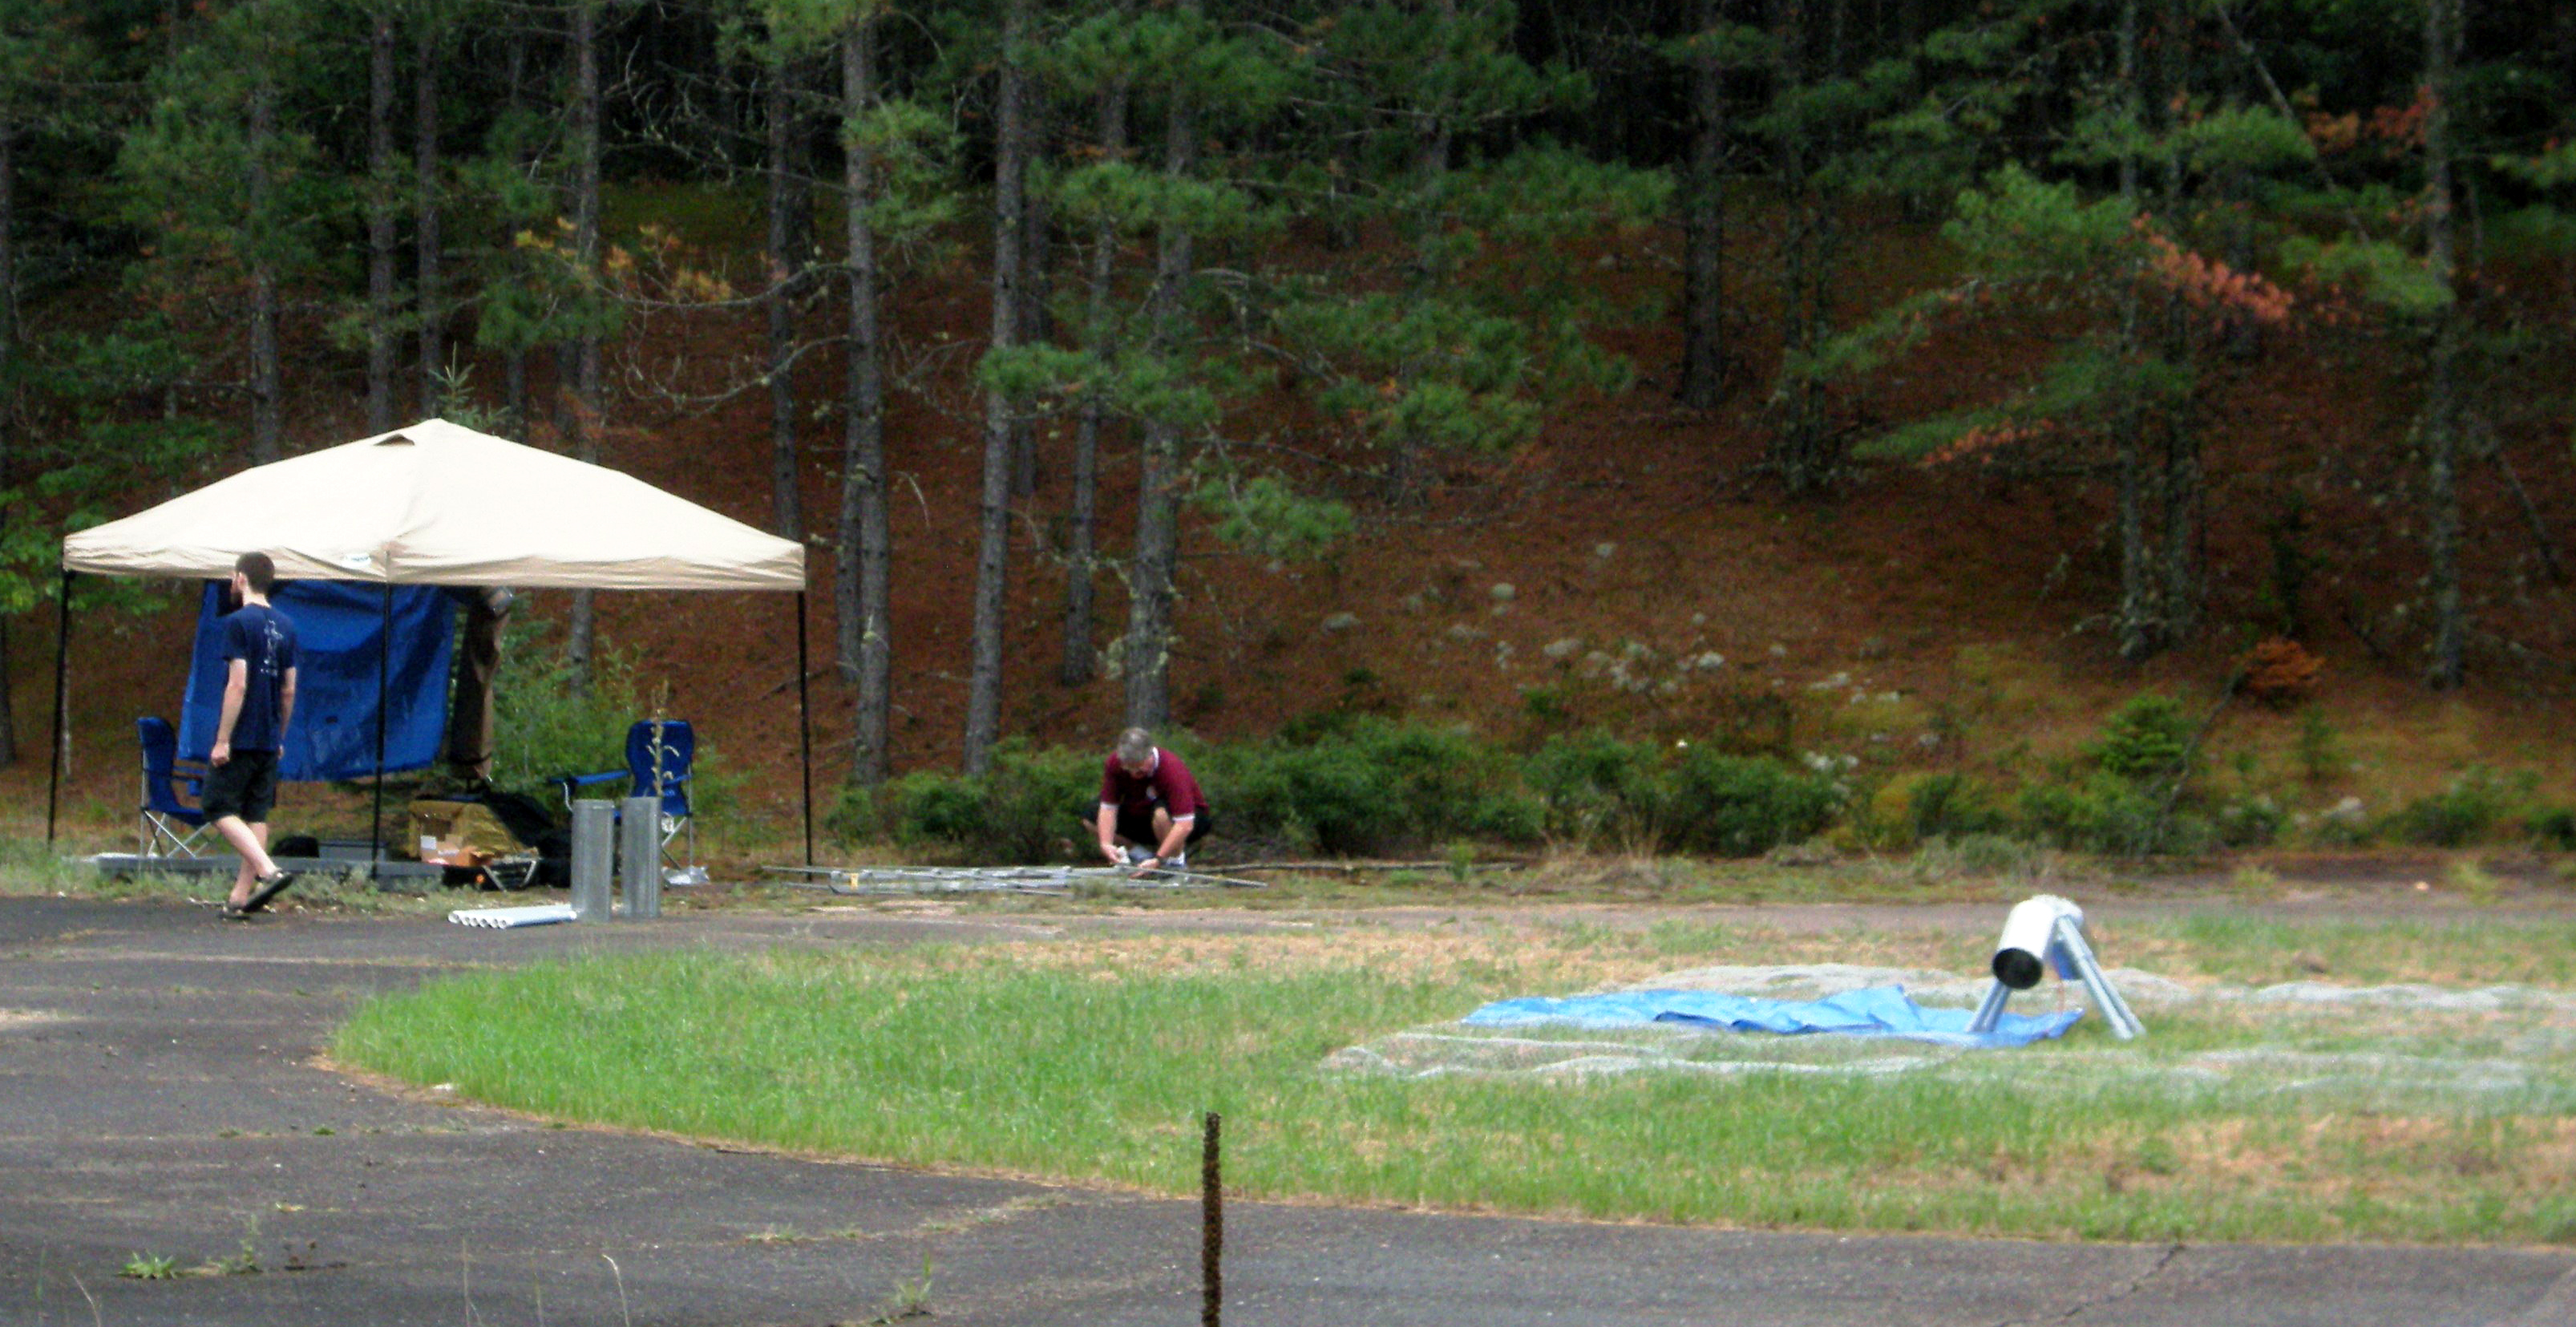
\includegraphics[width=0.95\linewidth]{SCIHI_system/figures/trombone_alg_sys.jpg}
\caption{SCI-HI setup with Trombone antenna on site at the Algonquin Radio Observatory in August 2012.}
\label{Fig:trombone_alg}
\end{minipage}%
\begin{minipage}[b]{0.02\textwidth}
\hspace{1cm}
\end{minipage}%
\begin{minipage}[b]{0.42\textwidth}
\centering
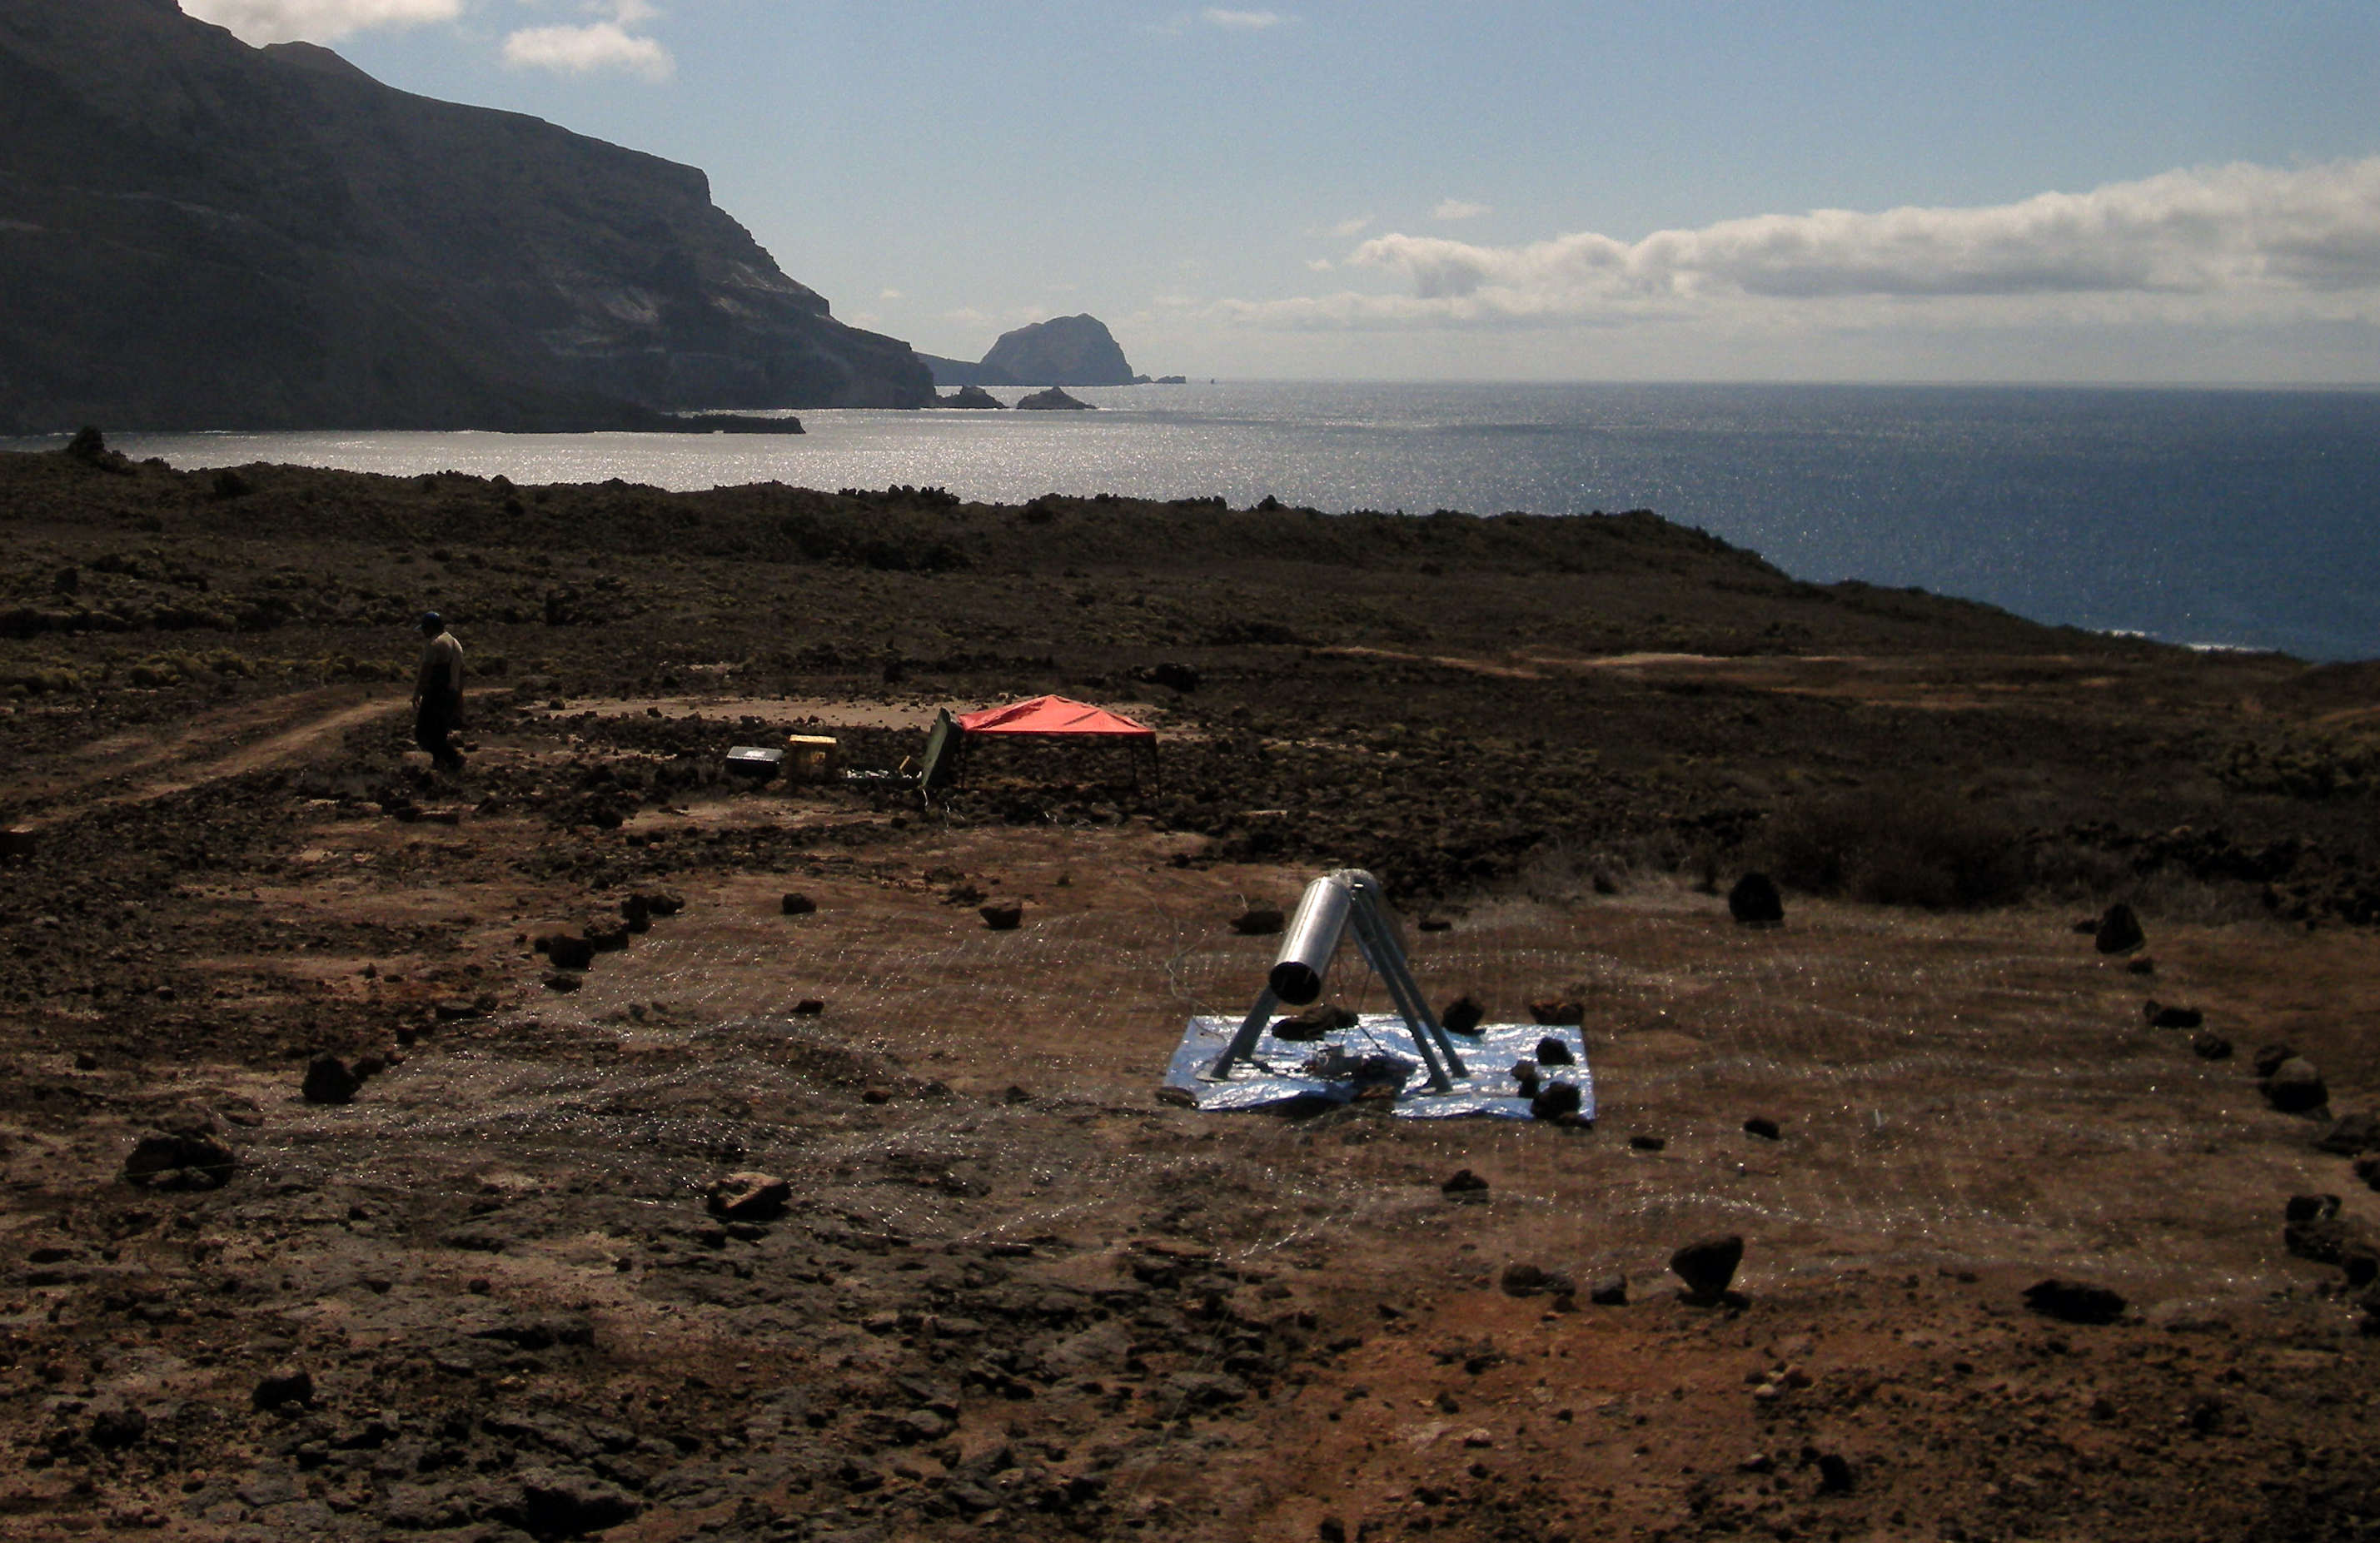
\includegraphics[width=0.95\linewidth]{SCIHI_system/figures/trombone_sys_guad.jpg}
\caption{SCI-HI setup with Trombone antenna on site at Isla Guadalupe in October 2012.}
\label{Fig:trombone_guad}
\end{minipage}
\end{figure}

\subsubsection{Antenna Deployment}

The Trombone antenna was used throughout the initial stages of the SCI-HI project. This included deployments at Green Bank in West Virginia (Figure \ref{Fig:trombone_gbt}), the Zona del Silencio in Mexico (Figure \ref{Fig:trombone_zds}), Algonquin Radio Observatory in Canada (Figure \ref{Fig:trombone_alg}), and Isla Guadalupe in Mexico (Figure \ref{Fig:trombone_guad}). For more discussion of these sites and why they were selected, see Chapter \ref{Ch:RFI}.

\begin{figure}[htb]
\centering
\begin{minipage}[b]{0.56\textwidth}
\centering
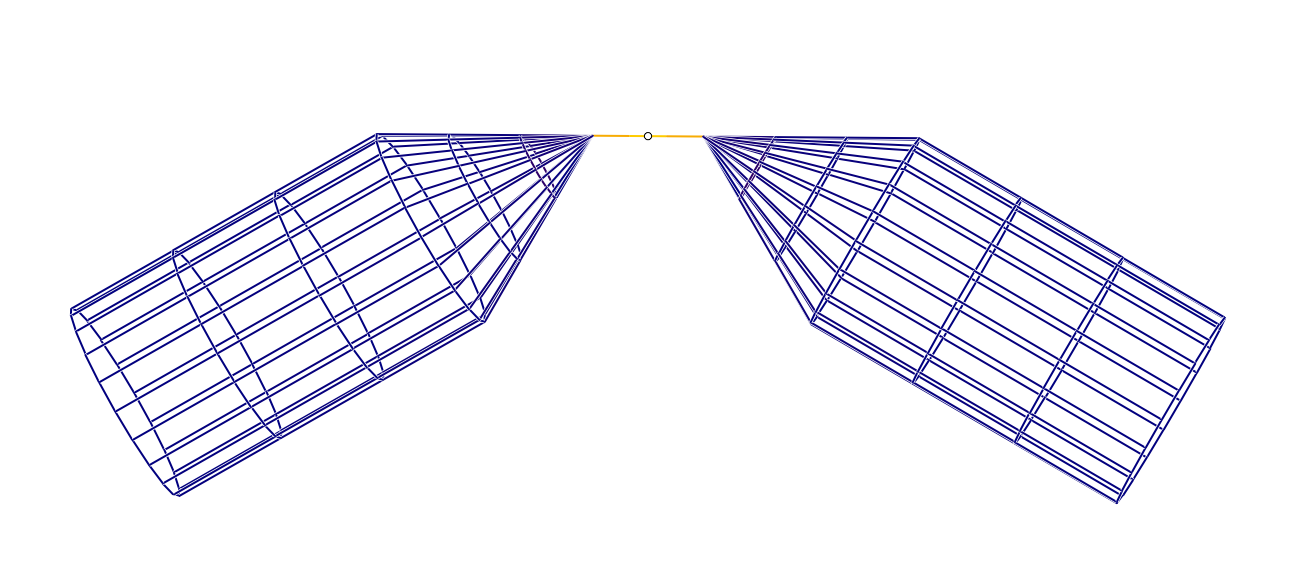
\includegraphics[width=0.95\linewidth]{SCIHI_system/figures/trombone_sim.png}
\caption{Simulated Trombone antenna design using cocoaNEC. Simulation software utilizes line segments which intersect to create structures. }
\label{Fig:trombone_sym}
\end{minipage}%
\begin{minipage}[b]{0.02\textwidth}
\hspace{1cm}
\end{minipage}%
\begin{minipage}[b]{0.42\textwidth}
\centering
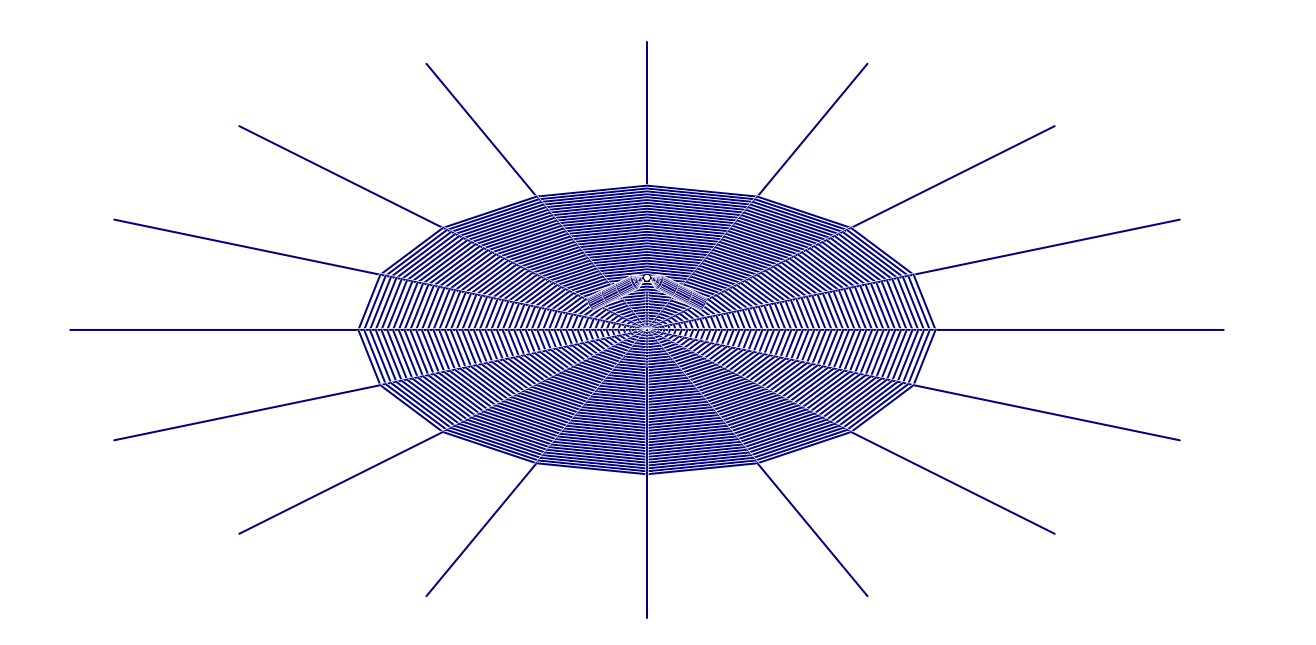
\includegraphics[width=0.95\linewidth]{SCIHI_system/figures/ground_plane_sim.png}
\caption{Circular ground plane with radials, simulated using cocoaNEC. The center, filled section has a $5 m$ radius and the radials extend an additional $5 m$.}
\label{Fig:gp_sym}
\end{minipage}
\end{figure}

\begin{figure}[htb]
\begin{center}
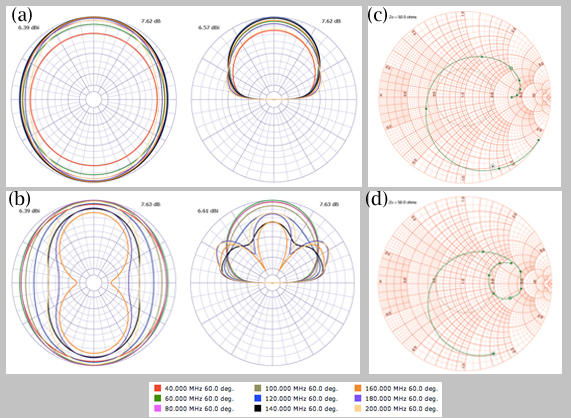
\includegraphics[width=0.95\linewidth]{SCIHI_system/figures/trombone_no_gp.jpg}
\caption{Trombone antenna simulation results with an idealized infinite ground plane. (a) Shows the azimuth (left) and elevation (right) antenna beam for different frequencies with the antenna at its shortest ($35 \; cm$) length. (b) Shows the same plots with the antenna at is longest ($86 \; cm$) length. (c) Shows a Smith chart of the antenna complex reflectivity ($S11$), where the 1.0 point corresponds to $Z = 50 \Omega$, for the shortest ($35 \; cm$) length. (d) Shows a Smith chart of the antenna complex reflectivity for the longest ($86 \; cm$) length. }
\label{Fig:trsym_nogp}
\end{center}
\end{figure}

\subsubsection{Antenna Simulation}

To better understand and assess the behavior of the Trombone antenna, simulations were run by Amy Stetten, a graduate student at CMU. Figure \ref{Fig:trombone_sym} shows the simulated Trombone design. Simulations were run using cocoaNEC,\footnote{\url{http://www.w7ay.net/site/Applications/cocoaNEC/}} a free antenna modelling code designed for use in a Macintosh OS environment. 

Simulations showed that the Trombone antenna beam was wide, but well behaved, for the shorter length as shown in Figure \ref{Fig:trsym_nogp}(a). In contrast, the longer length antenna beam had quite a bit of structure, as shown in Figure \ref{Fig:trsym_nogp}(b). In addition, the impedance of the antenna was not well matched to $50 \Omega$ and varied significantly across the band for all lengths (Figures \ref{Fig:trsym_nogp}(c) and \ref{Fig:trsym_nogp}(d)). 

\begin{figure}[htb]
\begin{center}
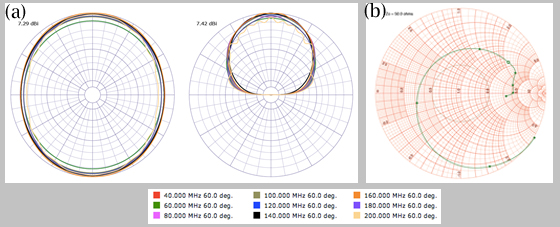
\includegraphics[width=0.95\linewidth]{SCIHI_system/figures/trombone_gp.jpg}
\caption{Trombone antenna simulation results with a spider web ground plane included in the simulation. (a) Shows the azimuth (left) and elevation (right) antenna beam for different frequencies with the antenna at its shortest ($35 \; cm$) length. (b) Shows a Smith chart of the antenna complex reflectivity, where 1.0 is set to $50 \Omega$, for the shortest ($35 \; cm$) length.}
\label{Fig:trsym_gp}
\end{center}
\end{figure}

Beyond the Trombone dipole antenna design, it was important to examine the effect of a non-ideal ground plane. Preliminary work with a square ground plane led to significant additional structure in the antenna beam. To counteract this structure, the ground plane was modified to the $''$spider-web$''$ design shown in Figure \ref{Fig:gp_sym}, with a center filled region and longer radials. 

Adding this style of ground plane to the system did not have a big impact on the simulation results (see Figure \ref{Fig:trsym_gp}) at most frequencies. There was additional structure in the beam at higher frequencies, but these frequencies are above the target frequency range of $40-130 MHz$.  

\begin{figure}[htb]
\centering
\begin{minipage}[b]{0.49\textwidth}
\centering
\includegraphics[width=0.95\linewidth]{SCIHI_system/figures/HIbiscus_top.png}
\caption{Simulated HIbiscus antenna as viewed from above.}
\label{Fig:HI_sim_top}
\end{minipage}%
\begin{minipage}[b]{0.02\textwidth}
\hspace{1cm}
\end{minipage}%
\begin{minipage}[b]{0.49\textwidth}
\centering
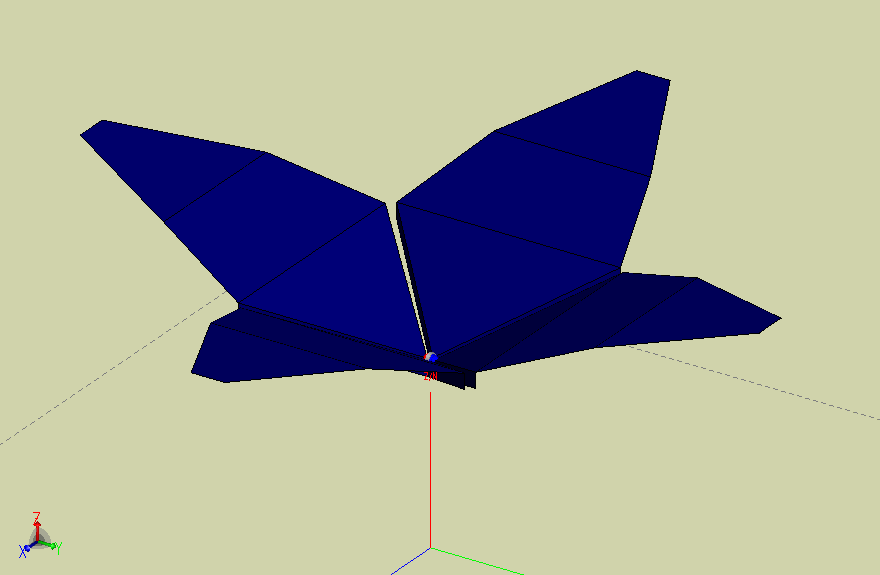
\includegraphics[width=0.95\linewidth]{SCIHI_system/figures/HIbiscus_ISO.png}
\caption{Simulated HIbiscus antenna as viewed from one side.}
\label{Fig:HI_sim_side}
\end{minipage}
\end{figure}


\begin{figure}[htb]
\centering
\begin{minipage}[b]{0.47\textwidth}
\centering
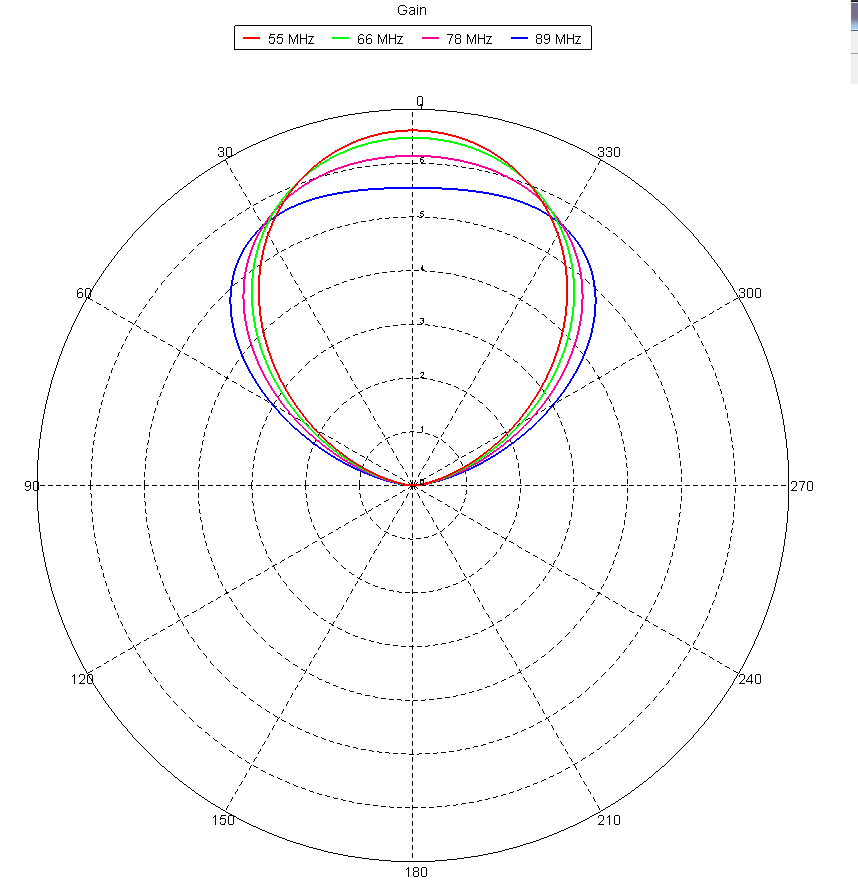
\includegraphics[width=0.95\linewidth]{SCIHI_system/figures/HIbiscus_sim_gain_beam1.png}
\caption{Simulated HIbiscus antenna beam slice in azimuth along the passive petals of the antenna (H-plane), shown for different frequencies.}
\label{Fig:HIsym_beam}
\end{minipage}%
\begin{minipage}[b]{0.02\textwidth}
\hspace{1cm}
\end{minipage}%
\begin{minipage}[b]{0.47\textwidth}
\centering
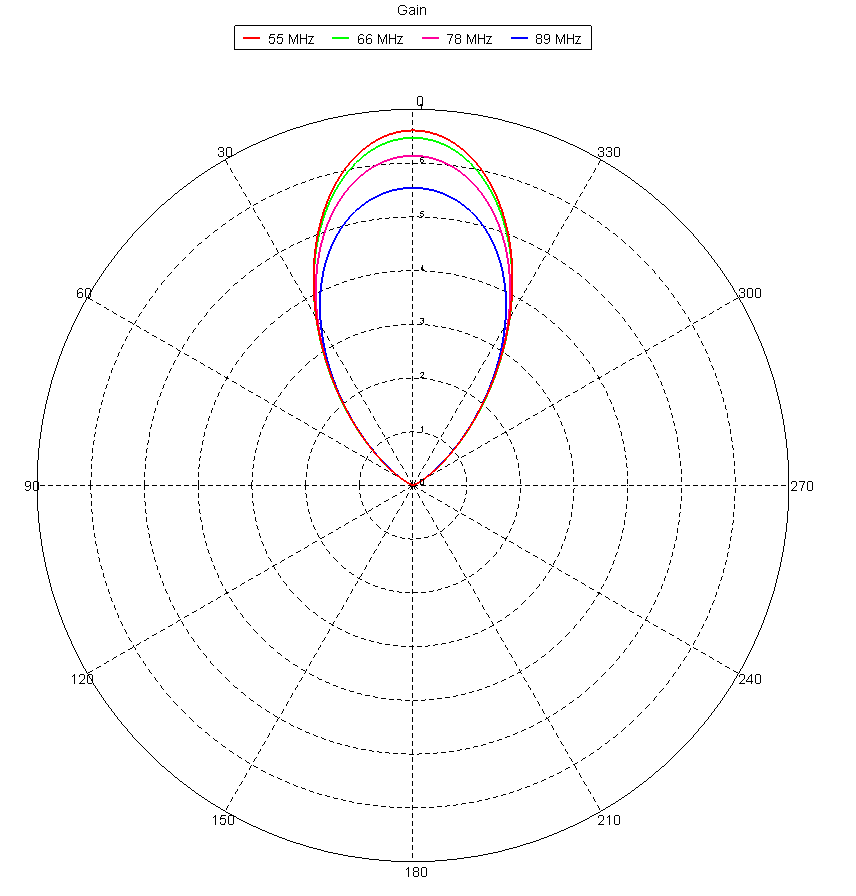
\includegraphics[width=0.95\linewidth]{SCIHI_system/figures/HIbiscus_sim_gain_beam2.png}
\caption{Simulated HIbiscus antenna beam slice in azimuth along the active petals of the antenna (E-plane), shown for different frequencies.}
\label{Fig:HIsym_beam_2}
\end{minipage}
\end{figure}
 
\begin{figure}[htb]
\centering
\begin{minipage}[b]{0.49\textwidth}
\centering
\includegraphics[width=0.95\linewidth]{SCIHI_system/figures/HIbiscus_S11_50_Cart.png}
\caption{Reflectivity of the simulated HIbiscus antenna when connected to a $50 \Omega$ transmission line. The narrow dip at $\sim 55 MHz$ is an antenna resonance. $S11$ is below -10 dB for a full octave of bandwidth.}
\label{Fig:HIsim_S11_dB}
\end{minipage}%
\begin{minipage}[b]{0.02\textwidth}
\hspace{1cm}
\end{minipage}%
\begin{minipage}[b]{0.46\textwidth}
\centering
\includegraphics[width=0.95\linewidth]{SCIHI_system/figures/HIbiscus_S11_50_Smith.png}
\caption{Smith chart of the simulated HIbiscus antenna complex $S11$ relative to $50 \Omega$ for $30 - 180 MHz$. The loop around the horizontal axis corresponds to frequencies with small $S11$. }
\label{Fig:HIsim_S11_Smith}
\end{minipage}
\end{figure}


\subsection{HIbiscus Antenna Design}

Simulation and testing demonstrated that the Trombone antenna has a wide beam and is not well behaved at higher frequencies. In addition, the impedance of the antenna is complex and strongly varying over our frequency band. 

Because of these problems, we decided to take our antenna design in a new direction. For this new direction, we started with a modified four-square antenna design used by the EDGES experiment \cite{bowman_2008}\cite{rogers_2008}, and modified it to fit our needs. Simulations were run by Jose-Miguel Juaregui-Garcia, a graduate student visiting CMU from INAOE. He ran the simulations using FEKO, a finite element computational electromagnetics software package.\footnote{\url{https://www.feko.info/}} 

Based on the FEKO simulation results, we settled on a design that used the EDGES design as a starting point, but changed the exact shapes of the four squares. We took each square and turned it into an inclined petal composed of three trapezoidal shapes. Each shape was connected to its neighbors on the petal, but had a different angle with respect to the ground. Additional panels were added to each side of the petal to create a strip line with a fixed gap between the petals. The entire antenna was then placed above a flat ground plane. We call this design a HIbiscus antenna, as shown in Figures \ref{Fig:HI_sim_top} and \ref{Fig:HI_sim_side}. 

This HIbiscus design has a $\sim 55^\circ$ full width half-maximum (FWHM) and no sidelobes over a wide frequency band, as shown in Figures \ref{Fig:HIsym_beam} and \ref{Fig:HIsym_beam_2}. The beam is narrower along the active elements (E-plane) of the antenna. The reflectivity of the HIbiscus antenna is complex, but is centered around $Z= 50 \Omega$ such that it has less than $-10 dB$ of reflectivity over a $60 MHz$ band. The complex structure of the simulated reflectivity is shown in Figure \ref{Fig:HIsim_S11_Smith}, and the magnitude of the simulated antenna reflectivity is shown in Figure \ref{Fig:HIsim_S11_dB}. 

\begin{figure}[htb]
\centering
\begin{minipage}[b]{0.52\textwidth}
\centering
\includegraphics[width=0.95\linewidth]{SCIHI_system/figures/model_test_tabitha.jpg}
\caption{One example of testing a scale model HIbiscus antenna in the CMU Project REAL Chamber. }
\label{Fig:hibiscus_scale_tabitha}
\end{minipage}%
\begin{minipage}[b]{0.02\textwidth}
\hspace{1cm}
\end{minipage}%
\begin{minipage}[b]{0.42\textwidth}
\centering
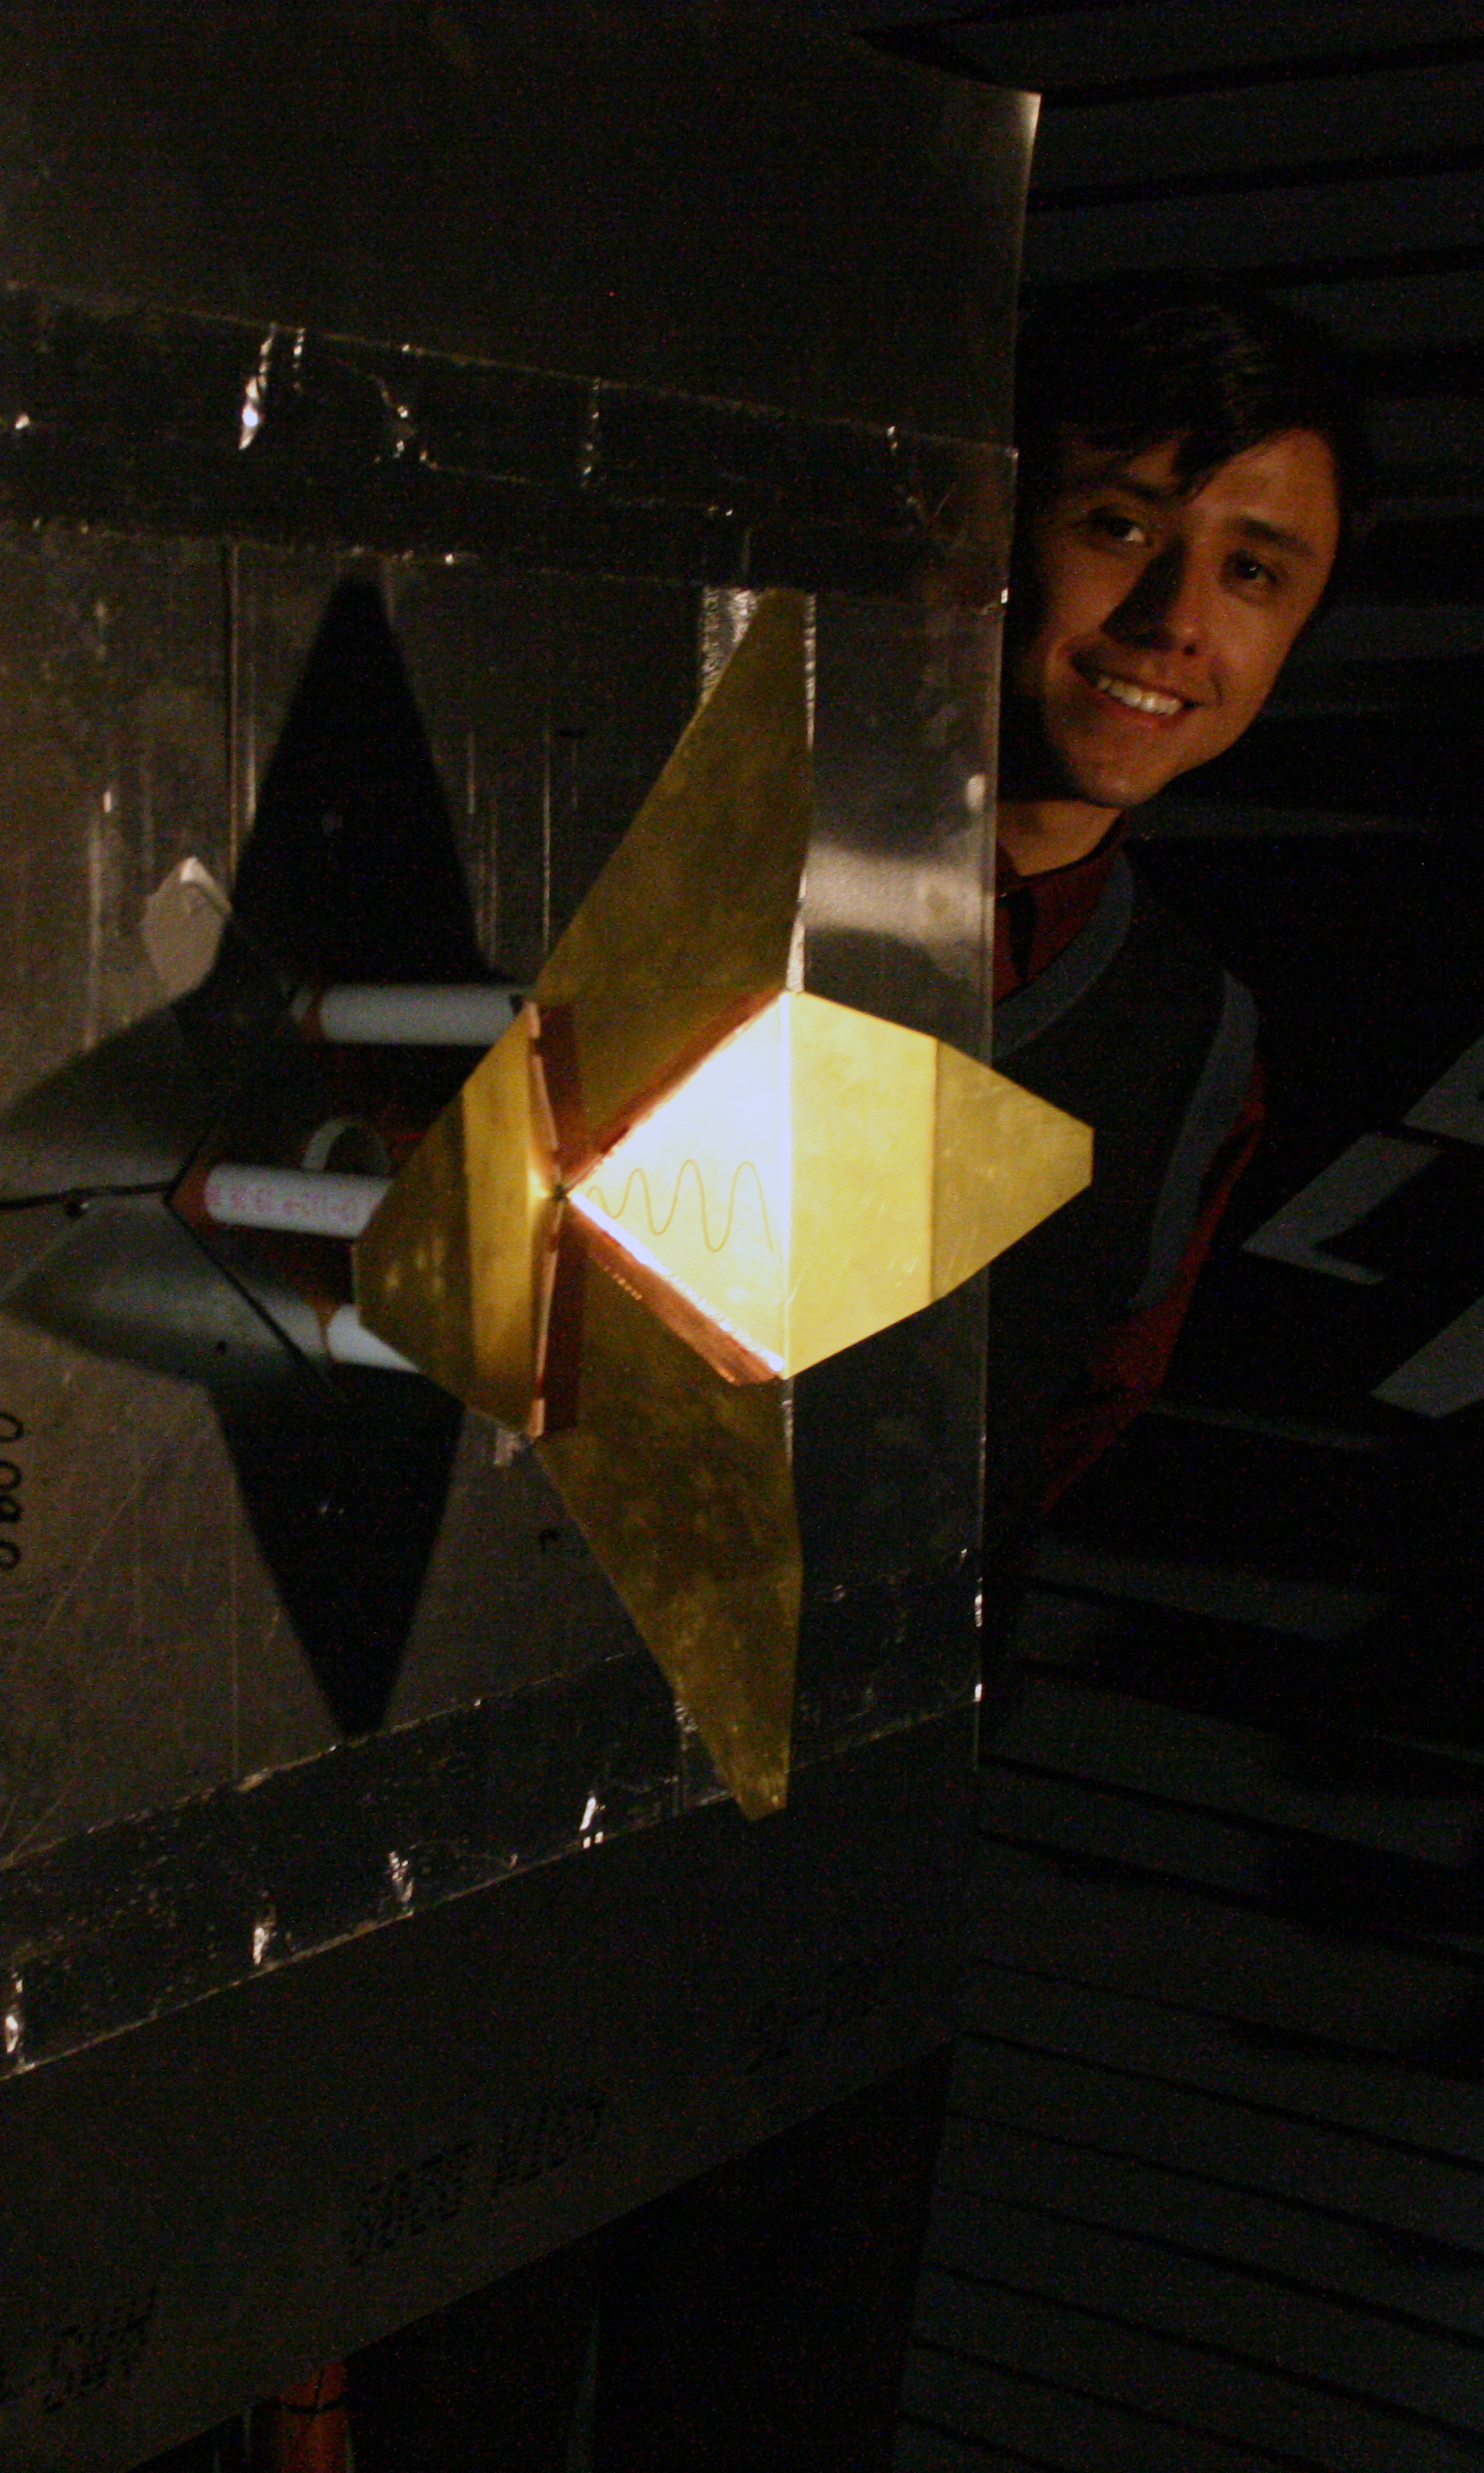
\includegraphics[width=0.95\linewidth]{SCIHI_system/figures/model_test_jose.jpg}
\caption{A second example of testing a scale model HIbiscus antenna in the CMU Project REAL Chamber.} 
\label{Fig:hibiscus_scale_jose}
\end{minipage}
\end{figure}
 
\begin{figure}[htb]
\centering
\begin{minipage}[b]{0.46\textwidth}
\centering
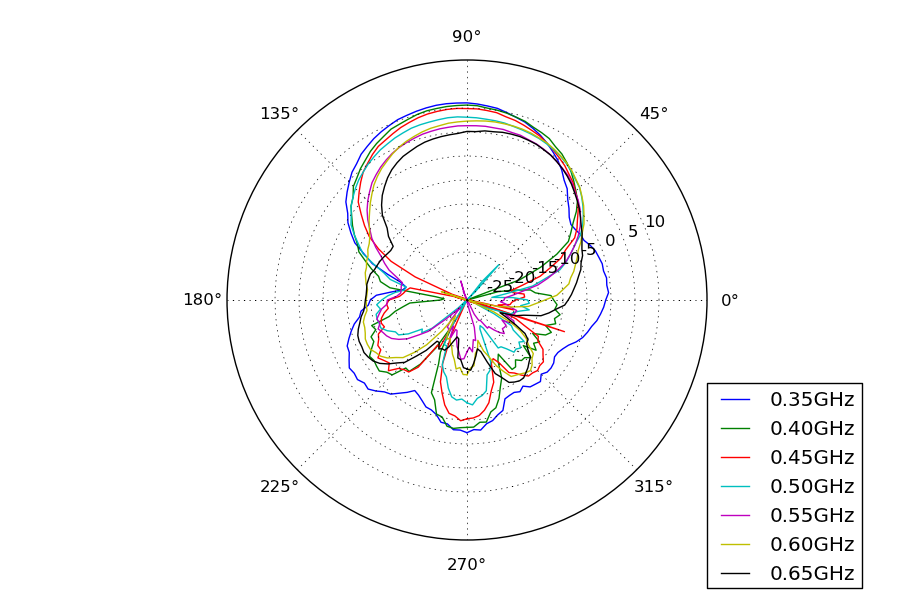
\includegraphics[width=0.95\linewidth]{SCIHI_system/figures/HIbiscus_Gain_model_H_polar.png}
\caption{Scale model antenna gain measured in the PREAL chamber. Data is taken along the plane of the dipole (active) petals of the antenna, the E-plane. }
\label{Fig:eplane_gain_sm}
\end{minipage}%
\begin{minipage}[b]{0.02\textwidth}
\hspace{1cm}
\end{minipage}%
\begin{minipage}[b]{0.48\textwidth}
\centering
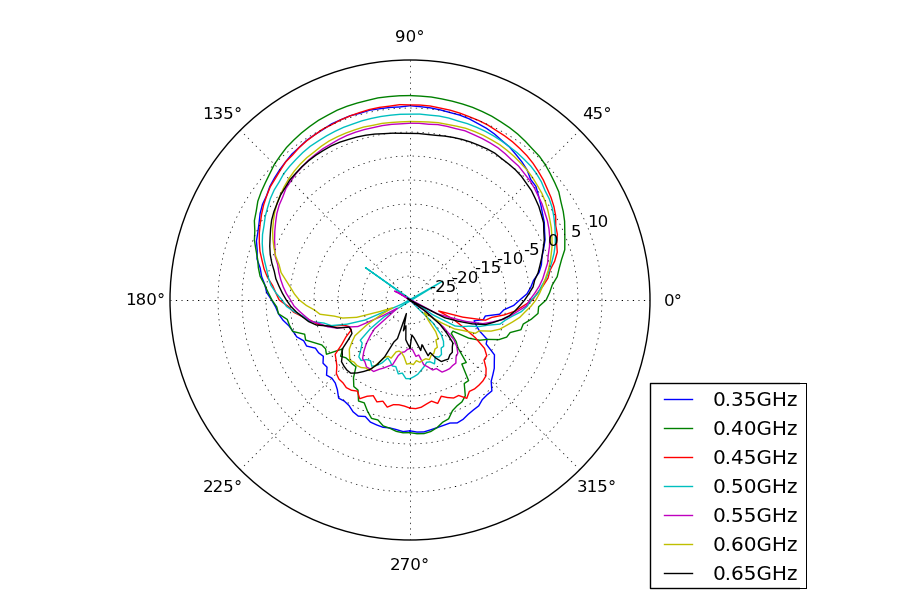
\includegraphics[width=0.95\linewidth]{SCIHI_system/figures/HIbiscus_Gain_model_V_polar.png}
\caption{Scale model antenna gain measured in the PREAL chamber. Data is taken perpendicular to the plane of the active petals of the antenna, the H-plane. }
\label{Fig:hplane_gain_sm}
\end{minipage}
\end{figure}

\begin{figure}[htb]
\centering
\begin{minipage}[b]{0.46\textwidth}
\centering
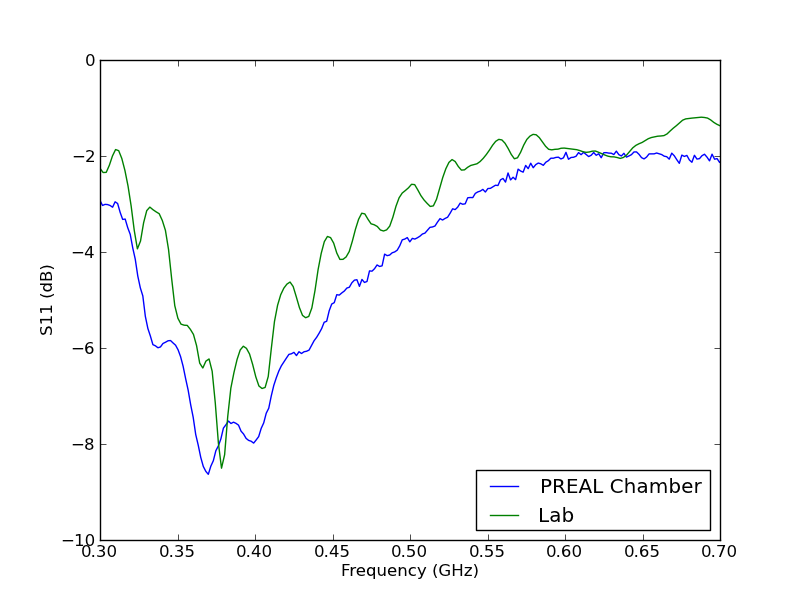
\includegraphics[width=0.95\linewidth]{SCIHI_system/figures/HIbiscus_S11_model_dB_PREAL.png}
\caption{Scale model antenna $S11$ reflectivity measured in the PREAL chamber and in the lab for the same model. Additional structure in the lab measurement comes from reflections off the walls of the lab.  }
\label{Fig:HIS11_model_dB}
\end{minipage}%
\begin{minipage}[b]{0.02\textwidth}
\hspace{1cm}
\end{minipage}%
\begin{minipage}[b]{0.48\textwidth}
\centering
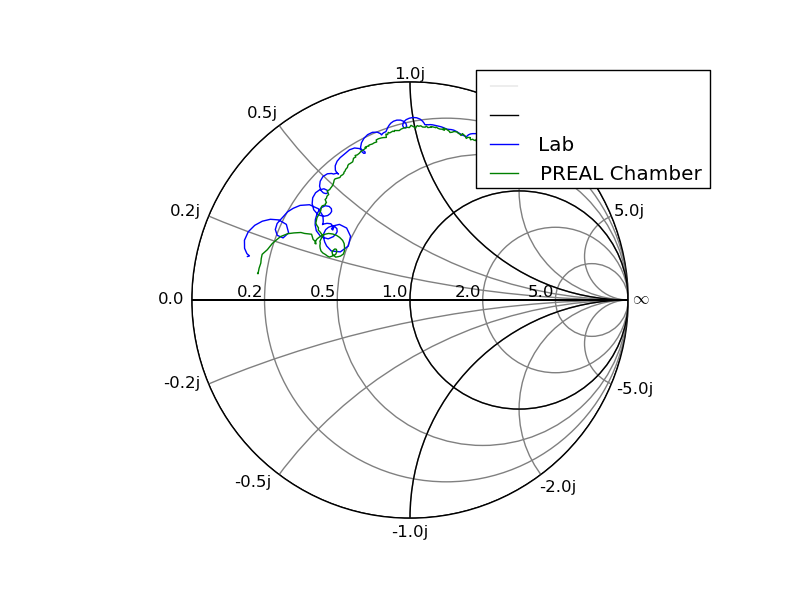
\includegraphics[width=0.95\linewidth]{SCIHI_system/figures/HIbiscus_S11_model_Smith_PREAL.png}
\caption{Scale model antenna $S11$ Smith chart as measured in the PREAL chamber and in the lab for one of the models. Frequency range for the data is $300-700 MHz$.}
\label{Fig:HIS11_model_Smith}
\end{minipage}
\end{figure}

\subsubsection{Scale Model Testing}

In order to test our simulation to see if it matched the real antenna performance, Jose-Miguel built a set of scaled HIbiscus designs tuned for higher frequencies around $400-500 MHz$. This allowed us to use an antenna range to measure the antenna beam shape and impedance. Jose-Miguel and I used the PREAL\footnote{\url{http://www.preal.ece.cmu.edu/}} (Project Remote Educational Antenna Laboratory) facility at Carnegie Mellon University to measure the antenna response of different scaled HIbiscus models. Figures \ref{Fig:hibiscus_scale_tabitha} and \ref{Fig:hibiscus_scale_jose} show two of the scale models being measured in the chamber.

Measuring scale models gave us the antenna gain for two azimuthal planes of the antenna. One, the E-plane, is along the active petals of the antenna. The other, the H-plane, is perpendicular to the E-plane and lies along the passive petals of the antenna. Figures \ref{Fig:eplane_gain_sm} and \ref{Fig:hplane_gain_sm} show the measured antenna gain for the scale model shown in Figure \ref{Fig:hibiscus_scale_tabitha}. Reflectivity of the scale model antenna was also measured using the PREAL facility, as shown in Figures \ref{Fig:HIS11_model_dB} and \ref{Fig:HIS11_model_Smith}

\begin{figure}[htb]
\centering
\begin{minipage}[b]{0.50\textwidth}
\centering
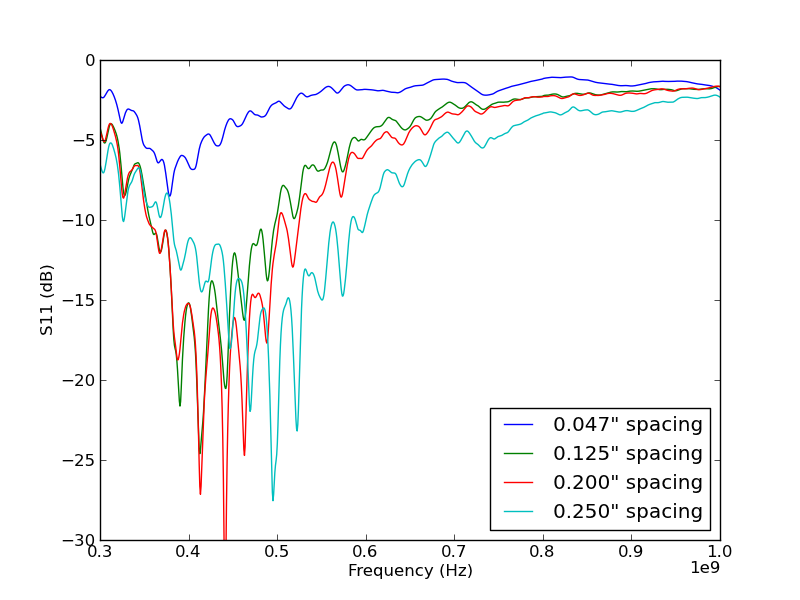
\includegraphics[width=0.95\linewidth]{SCIHI_system/figures/HIbiscus_S11_model_spacing_dB.png}
\caption{Scale model antenna $S11$ reflectivity measured in the lab for different strip line gap widths. Narrow features are due to reflections off the walls of the lab, while broad features show the actual reflectivity of the antenna. }
\label{Fig:HIS11_model_inc_dB}
\end{minipage}%
\begin{minipage}[b]{0.02\textwidth}
\hspace{1cm}
\end{minipage}%
\begin{minipage}[b]{0.46\textwidth}
\centering
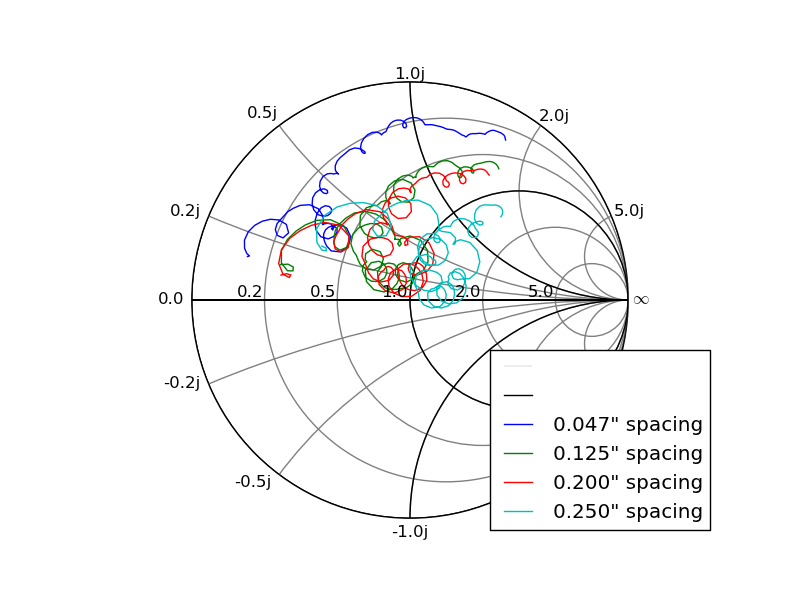
\includegraphics[width=0.95\linewidth]{SCIHI_system/figures/HIbiscus_S11_model_spacing_Smith.png}
\caption{Scale model antenna $S11$ Smith chart as measured in the lab for different strip line gap widths. Frequency range for the data is $300-700 MHz$. }
\label{Fig:HIS11_model_inc_Smith}
\end{minipage}
\end{figure}

Scale model testing indicated that antenna perfomance was particularly sensitive to two antenna shape parameters. These shape parameters are the strip line gap width and the height of the antenna with respect to the ground plane. Using measurements made after incremental adjustments of each parameter on one of the scale models, we optimized the antenna performance for our needs. Figures \ref{Fig:HIS11_model_inc_dB} and \ref{Fig:HIS11_model_inc_Smith} show one example of measurements made for incremental adjustments of the strip line gap width. 

One challenge of making $S11$ measurements is the presence of short period oscillations in the $S11$ data. These oscillations come from reflections off the walls of the lab where the $S11$ data was measured. Removing these oscillations requires a very large room with minimal reflection or outdoor measurements. Figures \ref{Fig:HIS11_model_dB} and \ref{Fig:HIS11_model_Smith} show a decrease in the magnitude of the oscillations when measurements were made using the PREAL chamber. This is because the chamber has lower reflection due to the anechoic foam on the chamber walls. 

Beyond the small scale oscillations, the large scale structure of the $S11$ measurement can be seen to shift as we change the strip line gap width. In the Smith chart (Figure \ref{Fig:HIS11_model_inc_Smith}) we see that changing the gap width moves the $S11$ data closer to the real axis and toward larger magnitude around 1.0 or $50 \Omega$. Using the scale model data, Jose-Miguel was also able to edit the antenna simulation to better match the actual antenna response. This gave us an excellent antenna model to use in our data analysis, as discussed in Chapter \ref{Ch:Data}. 

\begin{figure}[htb]
\centering
\begin{minipage}[b]{0.43\textwidth}
\centering
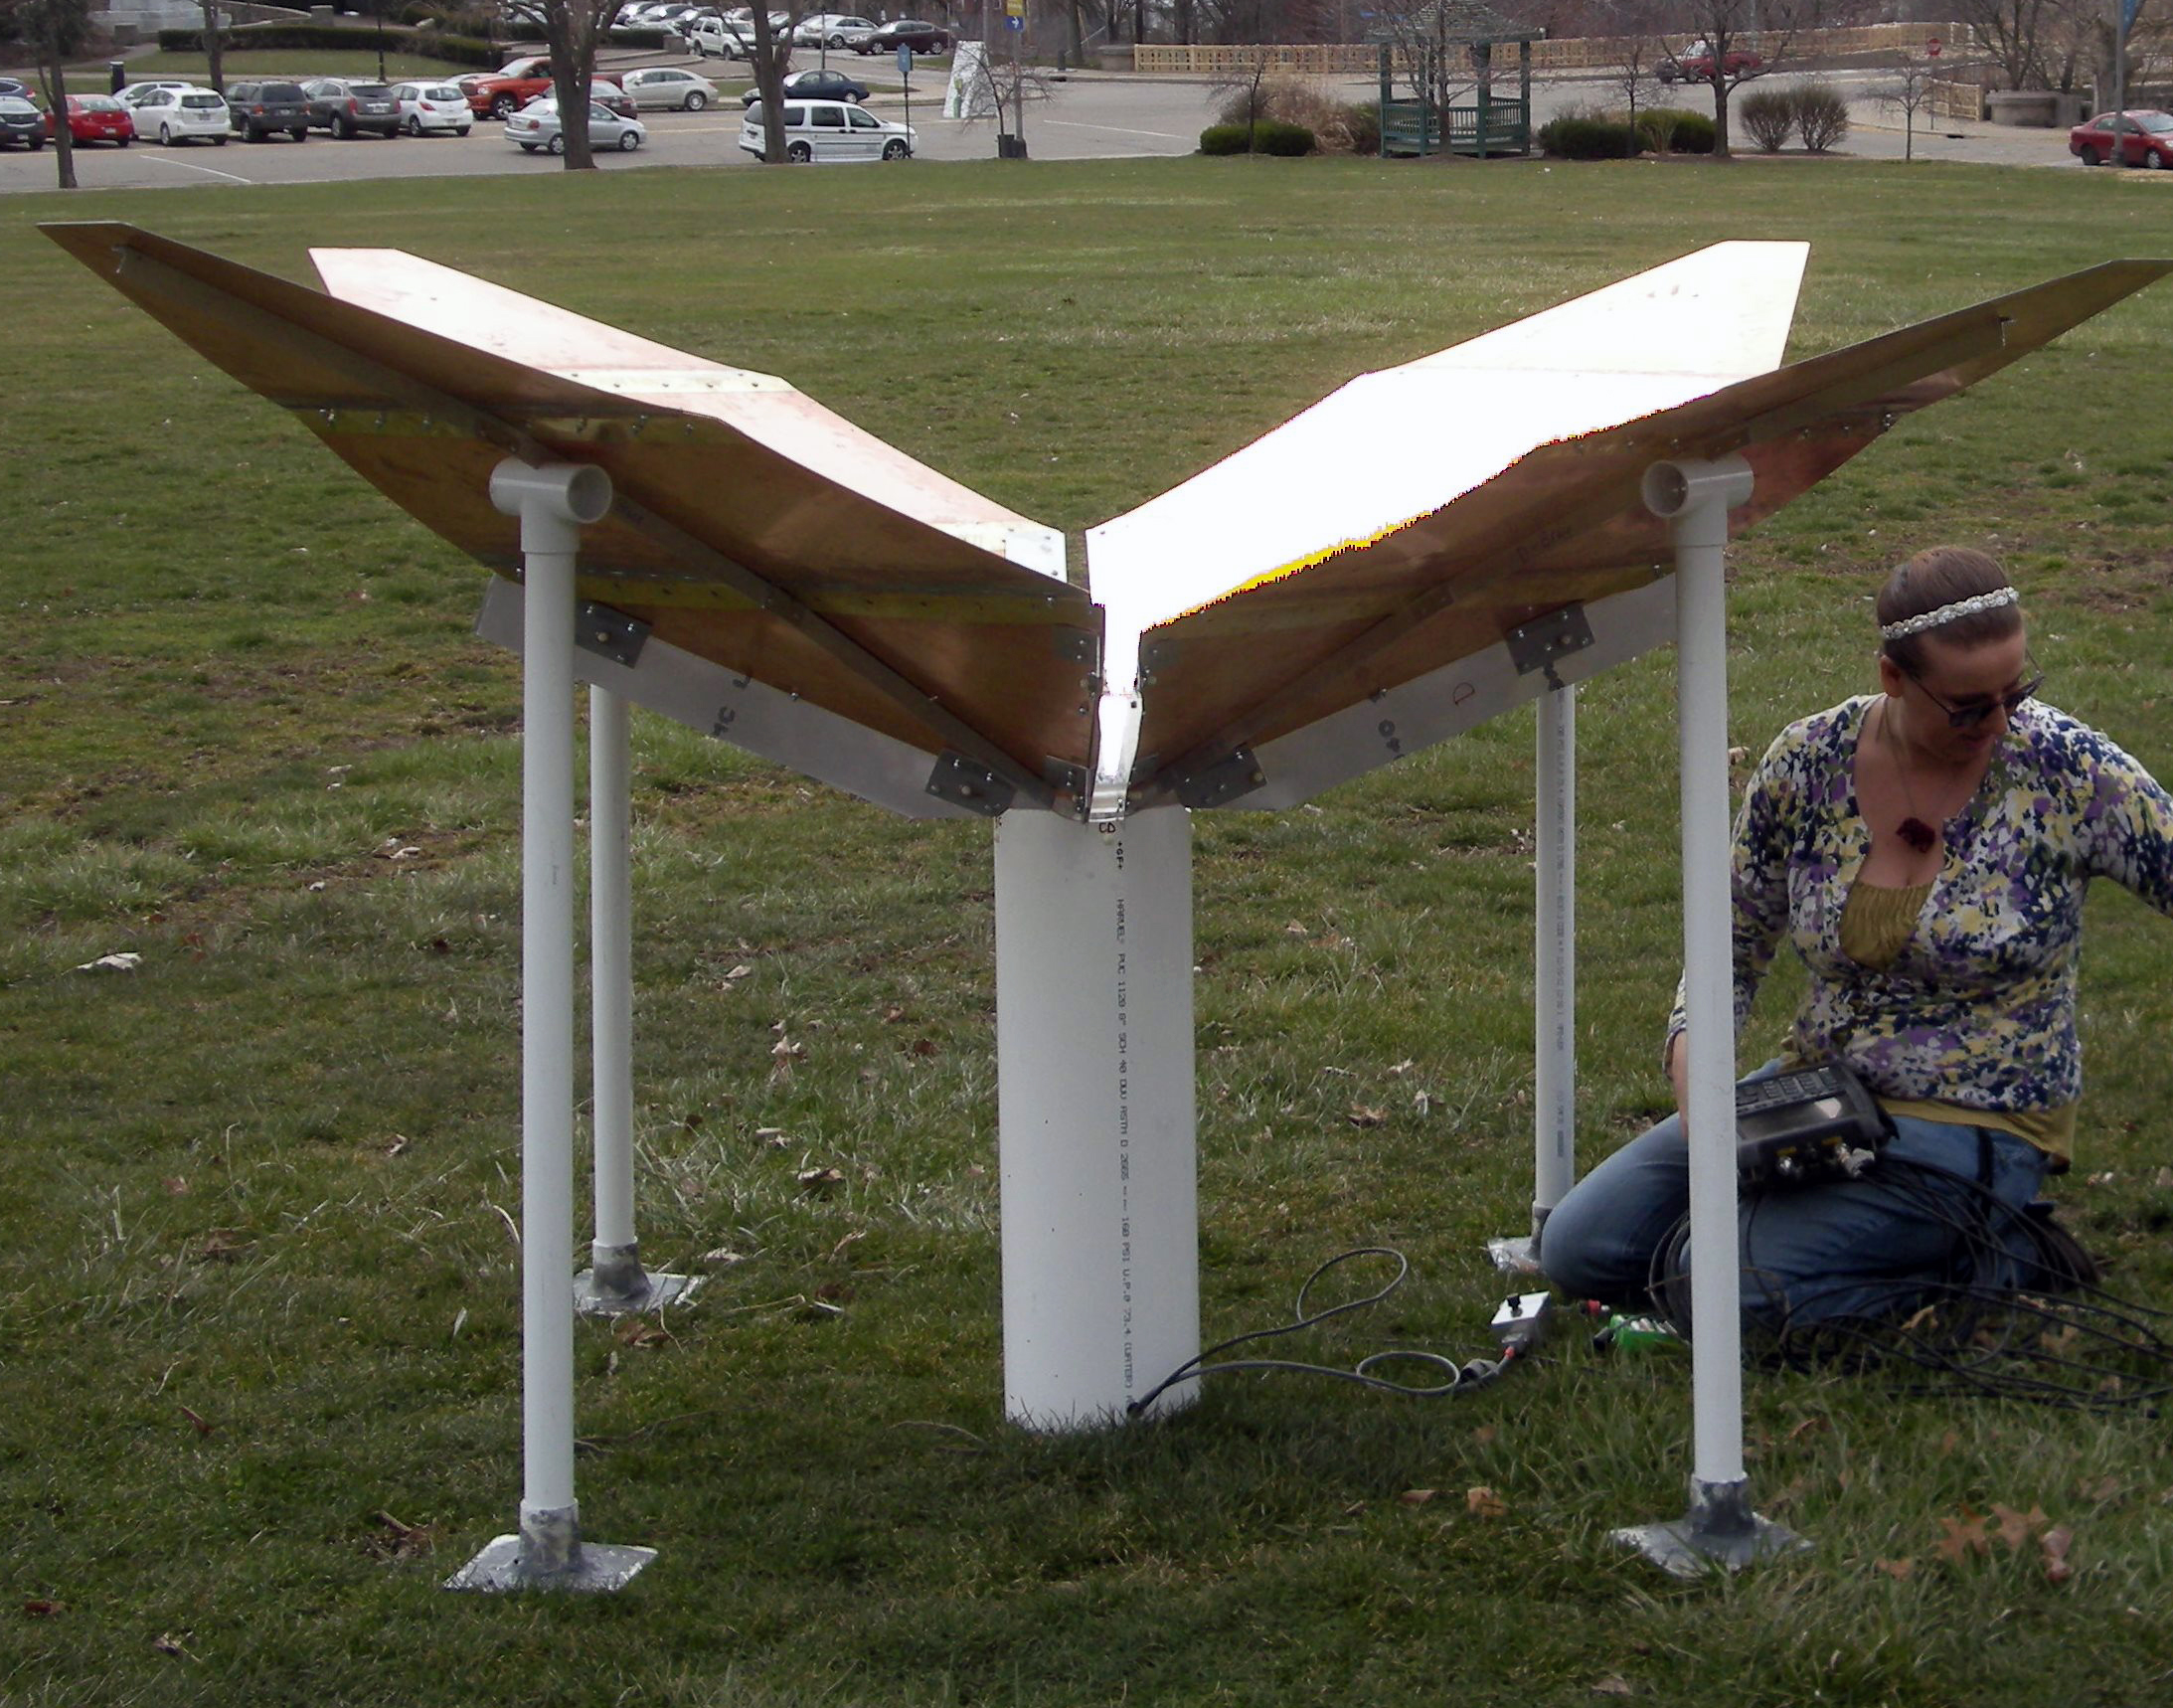
\includegraphics[width=0.95\linewidth]{SCIHI_system/figures/HIbiscus_pgh_imp.jpg}
\caption{HIbiscus antenna scaled for $70 MHz$ as it was set-up during S-parameter testing at CMU. }
\label{Fig:hibiscus_first}
\end{minipage}%
\begin{minipage}[b]{0.02\textwidth}
\hspace{1cm}
\end{minipage}%
\begin{minipage}[b]{0.51\textwidth}
\centering
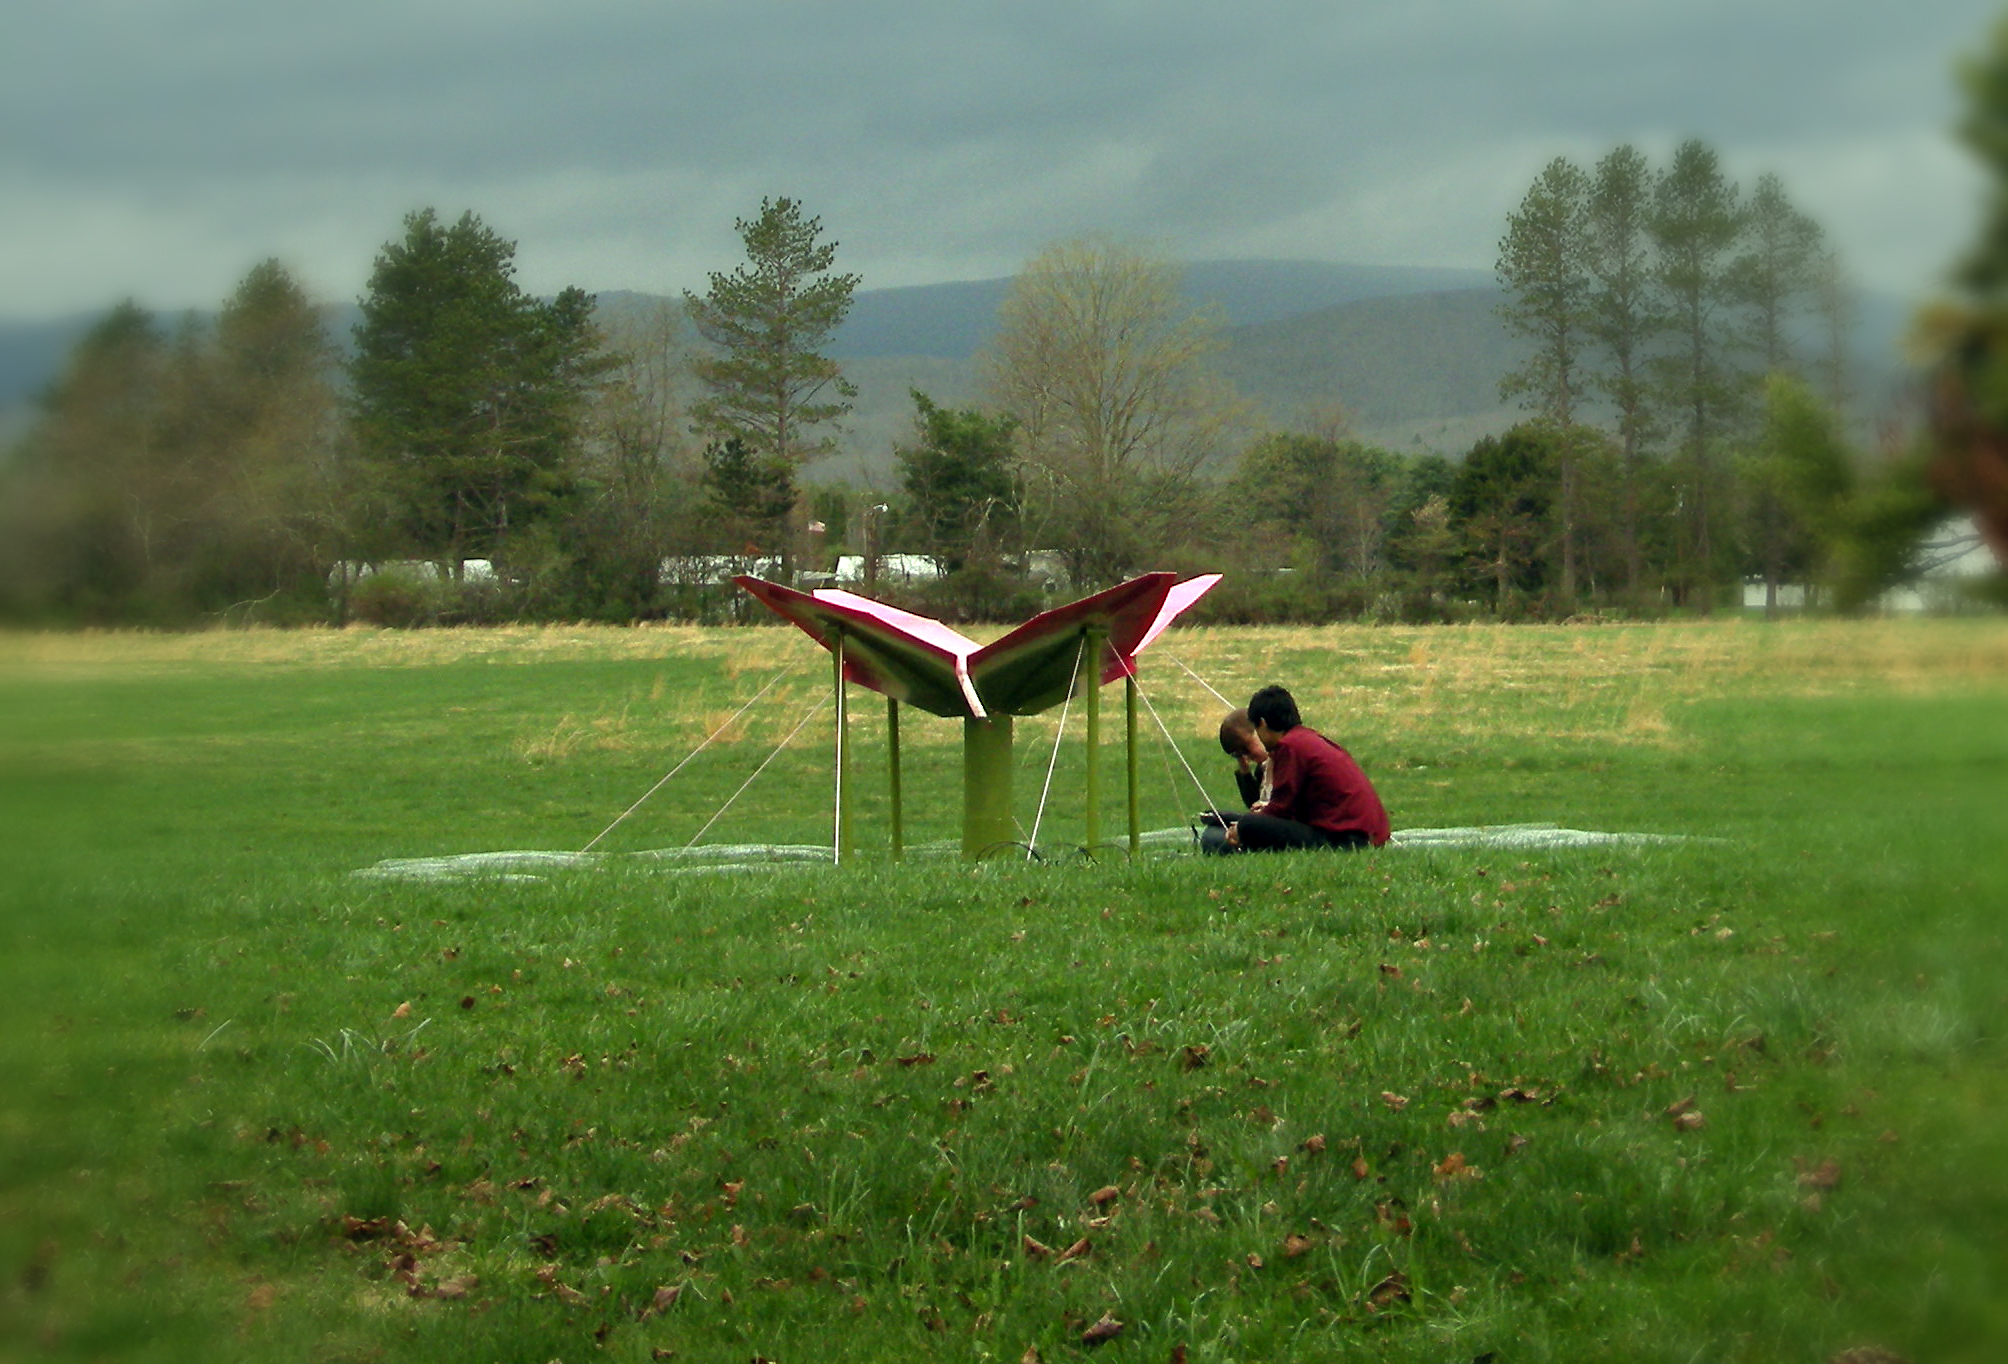
\includegraphics[width=0.95\linewidth]{SCIHI_system/figures/HIbiscus_gbt.jpg}
\caption{HIbiscus antenna scaled for $70 MHz$ set-up for S-parameter testing on site at Green Bank.}
\label{Fig:hibiscus_gbt}
\end{minipage}
\end{figure}


\subsection{HIbiscus Antenna Construction}

\subsubsection{Initial Assembly}

Once we had a design finalized, Jose-Miguel and I set out to construct a HIbiscus antenna with its center frequency tuned to $70 MHz$ (in the middle of the SCI-HI observation band).

Antenna petals were constructed in sections. To construct the antenna petals, large sheets of printed circuit board (PCB) material were used (see Figure \ref{Fig:hibiscus_pcb}). This material is double sided FR4-4 fiberglass sandwiched between two thin sheets of copper. Trapezoidal shapes were cut out of the large sheets, then brass flanges were added to connect the shapes. Underneath the center line of each petal we placed a rib made out of aluminum angle with the appropriate bends to match the angles between trapezoids. Finally, the strip line panels were added using brass sheets soldered to some of the trapezoids (see Figure \ref{Fig:hibiscus_solder}). The entire system is bolted together using screws, and can be separated into sections for travel. 

\begin{figure}[htb]
\centering
\begin{minipage}[b]{0.39\textwidth}
\centering
\includegraphics[width=0.95\linewidth]{SCIHI_system/figures/HIbiscus_pcb_cut.jpg}
\caption{HIbiscus antenna PCB panels being cut. }
\label{Fig:hibiscus_pcb}
\end{minipage}%
\begin{minipage}[b]{0.02\textwidth}
\hspace{1cm}
\end{minipage}%
\begin{minipage}[b]{0.55\textwidth}
\centering
\includegraphics[width=0.95\linewidth]{SCIHI_system/figures/HIbiscus_solder.jpg}
\caption{Soldering the strip line to the HIbiscus antenna panels.}
\label{Fig:hibiscus_solder}
\end{minipage}
\end{figure} 

The next step after petal construction was mounting of the petals. First, a small lucite mount was built for the connection points at the center of the antenna (see Figure \ref{Fig:hibiscus_center}). Next, lucite spacers were placed between each of the petals to keep the petal separation even and correct (see Figure \ref{Fig:hibiscus_spacer}). Finally, the entire system was raised above the ground using a set of five PVC pipe legs; a central column and one leg for each petal (see Figure \ref{Fig:hibiscus_first}). 

\begin{figure}[htb]
\centering
\begin{minipage}[b]{0.52\textwidth}
\centering
\includegraphics[width=0.95\linewidth]{SCIHI_system/figures/HIbiscus_strip_line.jpg}
\caption{Sight line down one of the strip lines for the HIbiscus antenna with spacers in place.}
\label{Fig:hibiscus_spacer}
\end{minipage}%
\begin{minipage}[b]{0.02\textwidth}
\hspace{1cm}
\end{minipage}%
\begin{minipage}[b]{0.42\textwidth}
\centering
\includegraphics[width=0.95\linewidth]{SCIHI_system/figures/HIbiscus_center_point.jpg}
\caption{Center of the HIbiscus antenna with spacers and center mount block in place.}
\label{Fig:hibiscus_center}
\end{minipage}
\end{figure}

Beyond the antenna structure, a ground plane was also required to avoid variation in the antenna pattern and impedance due to weather conditions. Like with the Trombone antenna, we used a ground plane made out of metal mesh (chicken wire). Using simulations we found that the HIbiscus antenna was not as sensitive to the shape of the ground plane. Simulations showed that a $\sim16 m^2$ square ground plane gave good results and and was easy to lay out. 

Weather-proofing was also important for the design. The entire system (antenna plus ground plane) was anchored to the ground to minimize the wind impact. Each of the four support legs had an anchoring rope (see Figure \ref{Fig:hibiscus_gbt}), and the chicken wire was anchored with many small stakes. This had the added advantage of keeping the ground plane flat to the ground. 

\begin{figure}[htb]
\centering
\begin{minipage}[b]{0.53\textwidth}
\centering
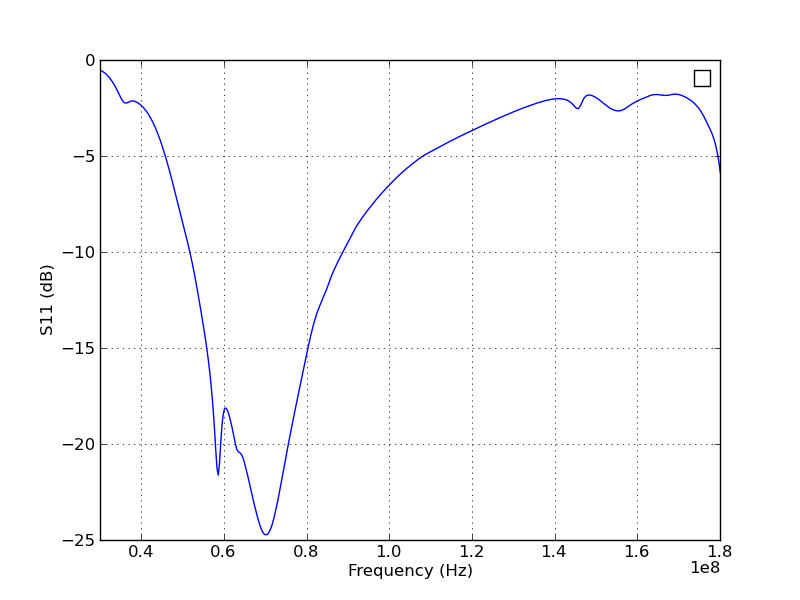
\includegraphics[width=0.95\linewidth]{SCIHI_system/figures/HIbiscus_S11_dB_70MHz.png}
\caption{Measured HIbiscus antenna $S11$ reflectivity for antenna on-site at Isla Guadalupe. }
\label{Fig:HIS11_dB_70}
\end{minipage}%
\begin{minipage}[b]{0.02\textwidth}
\hspace{1cm}
\end{minipage}%
\begin{minipage}[b]{0.44\textwidth}
\centering
\includegraphics[width=0.95\linewidth]{SCIHI_system/figures/HIbiscus_S11_meas_smith.png}
\caption{Measured HIbiscus antenna $S11$ Smith chart for $30-200 MHz$ measured on-site at Isla Guadalupe. Loop around 1.0 corresponds to frequencies with minimum $S11$ magnitude.}
\label{Fig:HIS11_Smith_70}
\end{minipage}
\end{figure}

\subsubsection{S-parameters and Impedance}\label{Sec:HIbiscus_Imp}

Following antenna construction, reflectivity was measured for the full size antenna. This allowed us to compare the full size results to the scale model measurements. I set up the antenna outdoors and made measurements with a portable Vector Network Analyzer (VNA). Measurements had to be made outdoors to avoid having signal reflections from the walls of a room interfere with the results. We saw this previously with the scale model testing, and the longer wavelengths ($\sim 1-10 m$) of the SCI-HI band make reflections an even larger problem. Figures \ref{Fig:hibiscus_first} and \ref{Fig:hibiscus_gbt} show examples of how I made this measurement at CMU and Green Bank with the help of Jose-Miguel and others.

The full size HIbiscus $S11$ measurement is shown in Figures \ref{Fig:HIS11_dB_70} and \ref{Fig:HIS11_Smith_70}. Data for the figures was collected on-site at Isla Guadalupe with the antenna ground plane in place. We can compare this measurement to the simulated reflectivity shown in Figure \ref{Fig:HIsim_S11_dB}. The simulation successfully identified the antenna resonance between $50-60 MHz$ and the overall shape of the antenna reflectivity matches the simulation. Like in the scale model data shown in Figures \ref{Fig:HIS11_model_dB} and \ref{Fig:HIS11_model_inc_dB}, the minimum reflectivity magnitude is much lower than the simulation predicts. 

\begin{figure}[htb]
\centering
\begin{minipage}[b]{0.50\textwidth}
\centering
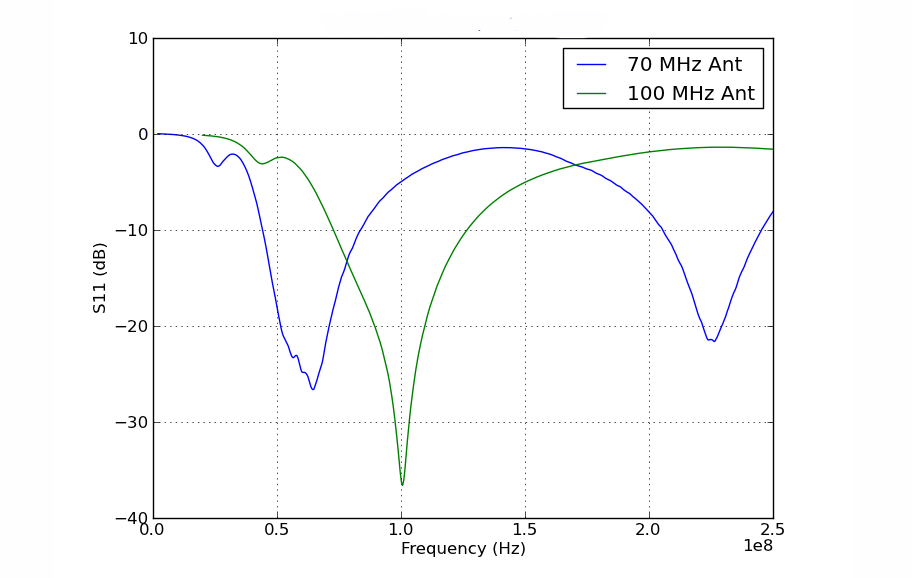
\includegraphics[width=0.95\linewidth]{SCIHI_system/figures/HIbiscus_S11_dB_both.png}
\caption{Measured HIbiscus $S11$ reflectivity for new antennas scaled for $70 MHz$ and $100 MHz$. Measurements were made without the ground plane in place. }
\label{Fig:HIS11_dB}
\end{minipage}%
\begin{minipage}[b]{0.02\textwidth}
\hspace{1cm}
\end{minipage}%
\begin{minipage}[b]{0.46\textwidth}
\centering
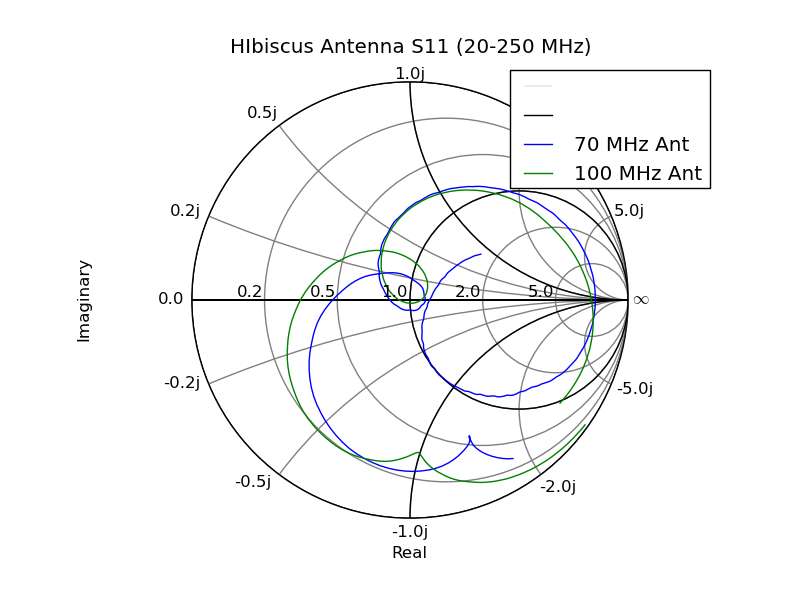
\includegraphics[width=0.95\linewidth]{SCIHI_system/figures/HIbiscus_S11_Smith_both.png}
\caption{Measured Smith chart for the HIbiscus antennas scaled for $70 MHz$ and $100 MHz$ without the ground plane in place.}
\label{Fig:HIS11_Smith}
\end{minipage}
\end{figure}

When the antenna was upgraded, as will be described later in this section, we again measured the $S11$ data for the antennas scaled to $70 MHz$ and $100 MHz$. These measurements assessed the new antennas and checked that they match expectations. $S11$ measurements for the new antennas are shown in Figures \ref{Fig:HIS11_dB} and \ref{Fig:HIS11_Smith}. 

From the magnitude of the reflectivity in Figure \ref{Fig:HIS11_dB} we see that measurement without the ground plane in the system removes the antenna resonance around $55 MHz$. Meanwhile, the overall shape of the reflectivity matches the earlier antenna. Also as expected, the $100 MHz$ antenna reflectivity looks like a scaled version of the $70 MHz$ antenna reflectivity. Complex structure of the antenna reflectivity, shown in the Smith chart in Figure \ref{Fig:HIS11_Smith}, also matches past measurements and simulation. The loop around $50 \Omega$ corresponds to frequencies where the reflectivity is at a minimum. 

\subsubsection{Travelling with the Antenna}

In order to use the HIbiscus antenna on-site at remote locations, it needs to be transportable to those locations and easily assembled upon arrival. Design of the mechanical structure of the antenna incorporated techniques that allowed us to meet this requirement. 

First, the entire antenna structure is very lightweight. This is because we built the antenna petals out of PCB material, which has the stiffness of sheet metal without the weight.  

Second, we laid out each of the antenna petals as a series of flat panels that can be easily assembled into a full petal or packed away into small bags. Each petal separats out into three trapezoids that screwed together for assembly, but could be packed as mostly flat sheets. The lucite spacers between the petals are mounted using nylon screws, while the central mount uses metal screws to attach the petals to a short piece of coaxial cable. Both can be assembled or disassembled and packed rapidly. The PVC pipe supports are also mounted using screws and can be rapidly assembled or disassembled and packed. 

Third, the entire antenna structure is small and light enough that it can be packed up into three suitcases plus an extra bag for the ground plane chicken wire. These suitcases meet the limitations for regular checked baggage on commercial airlines. 

\begin{figure}[htb]
\begin{center}
\includegraphics[width=0.95\linewidth]{SCIHI_system/figures/HIbiscus_70mhz_lab.jpg}
\caption{New HIbiscus antenna scaled for $70 MHz$ as laid out in the lab. Scale model in picture for comparison.}
\label{Fig:hibiscus_70}
\end{center}
\end{figure}

\begin{figure}[htb]
\begin{center}
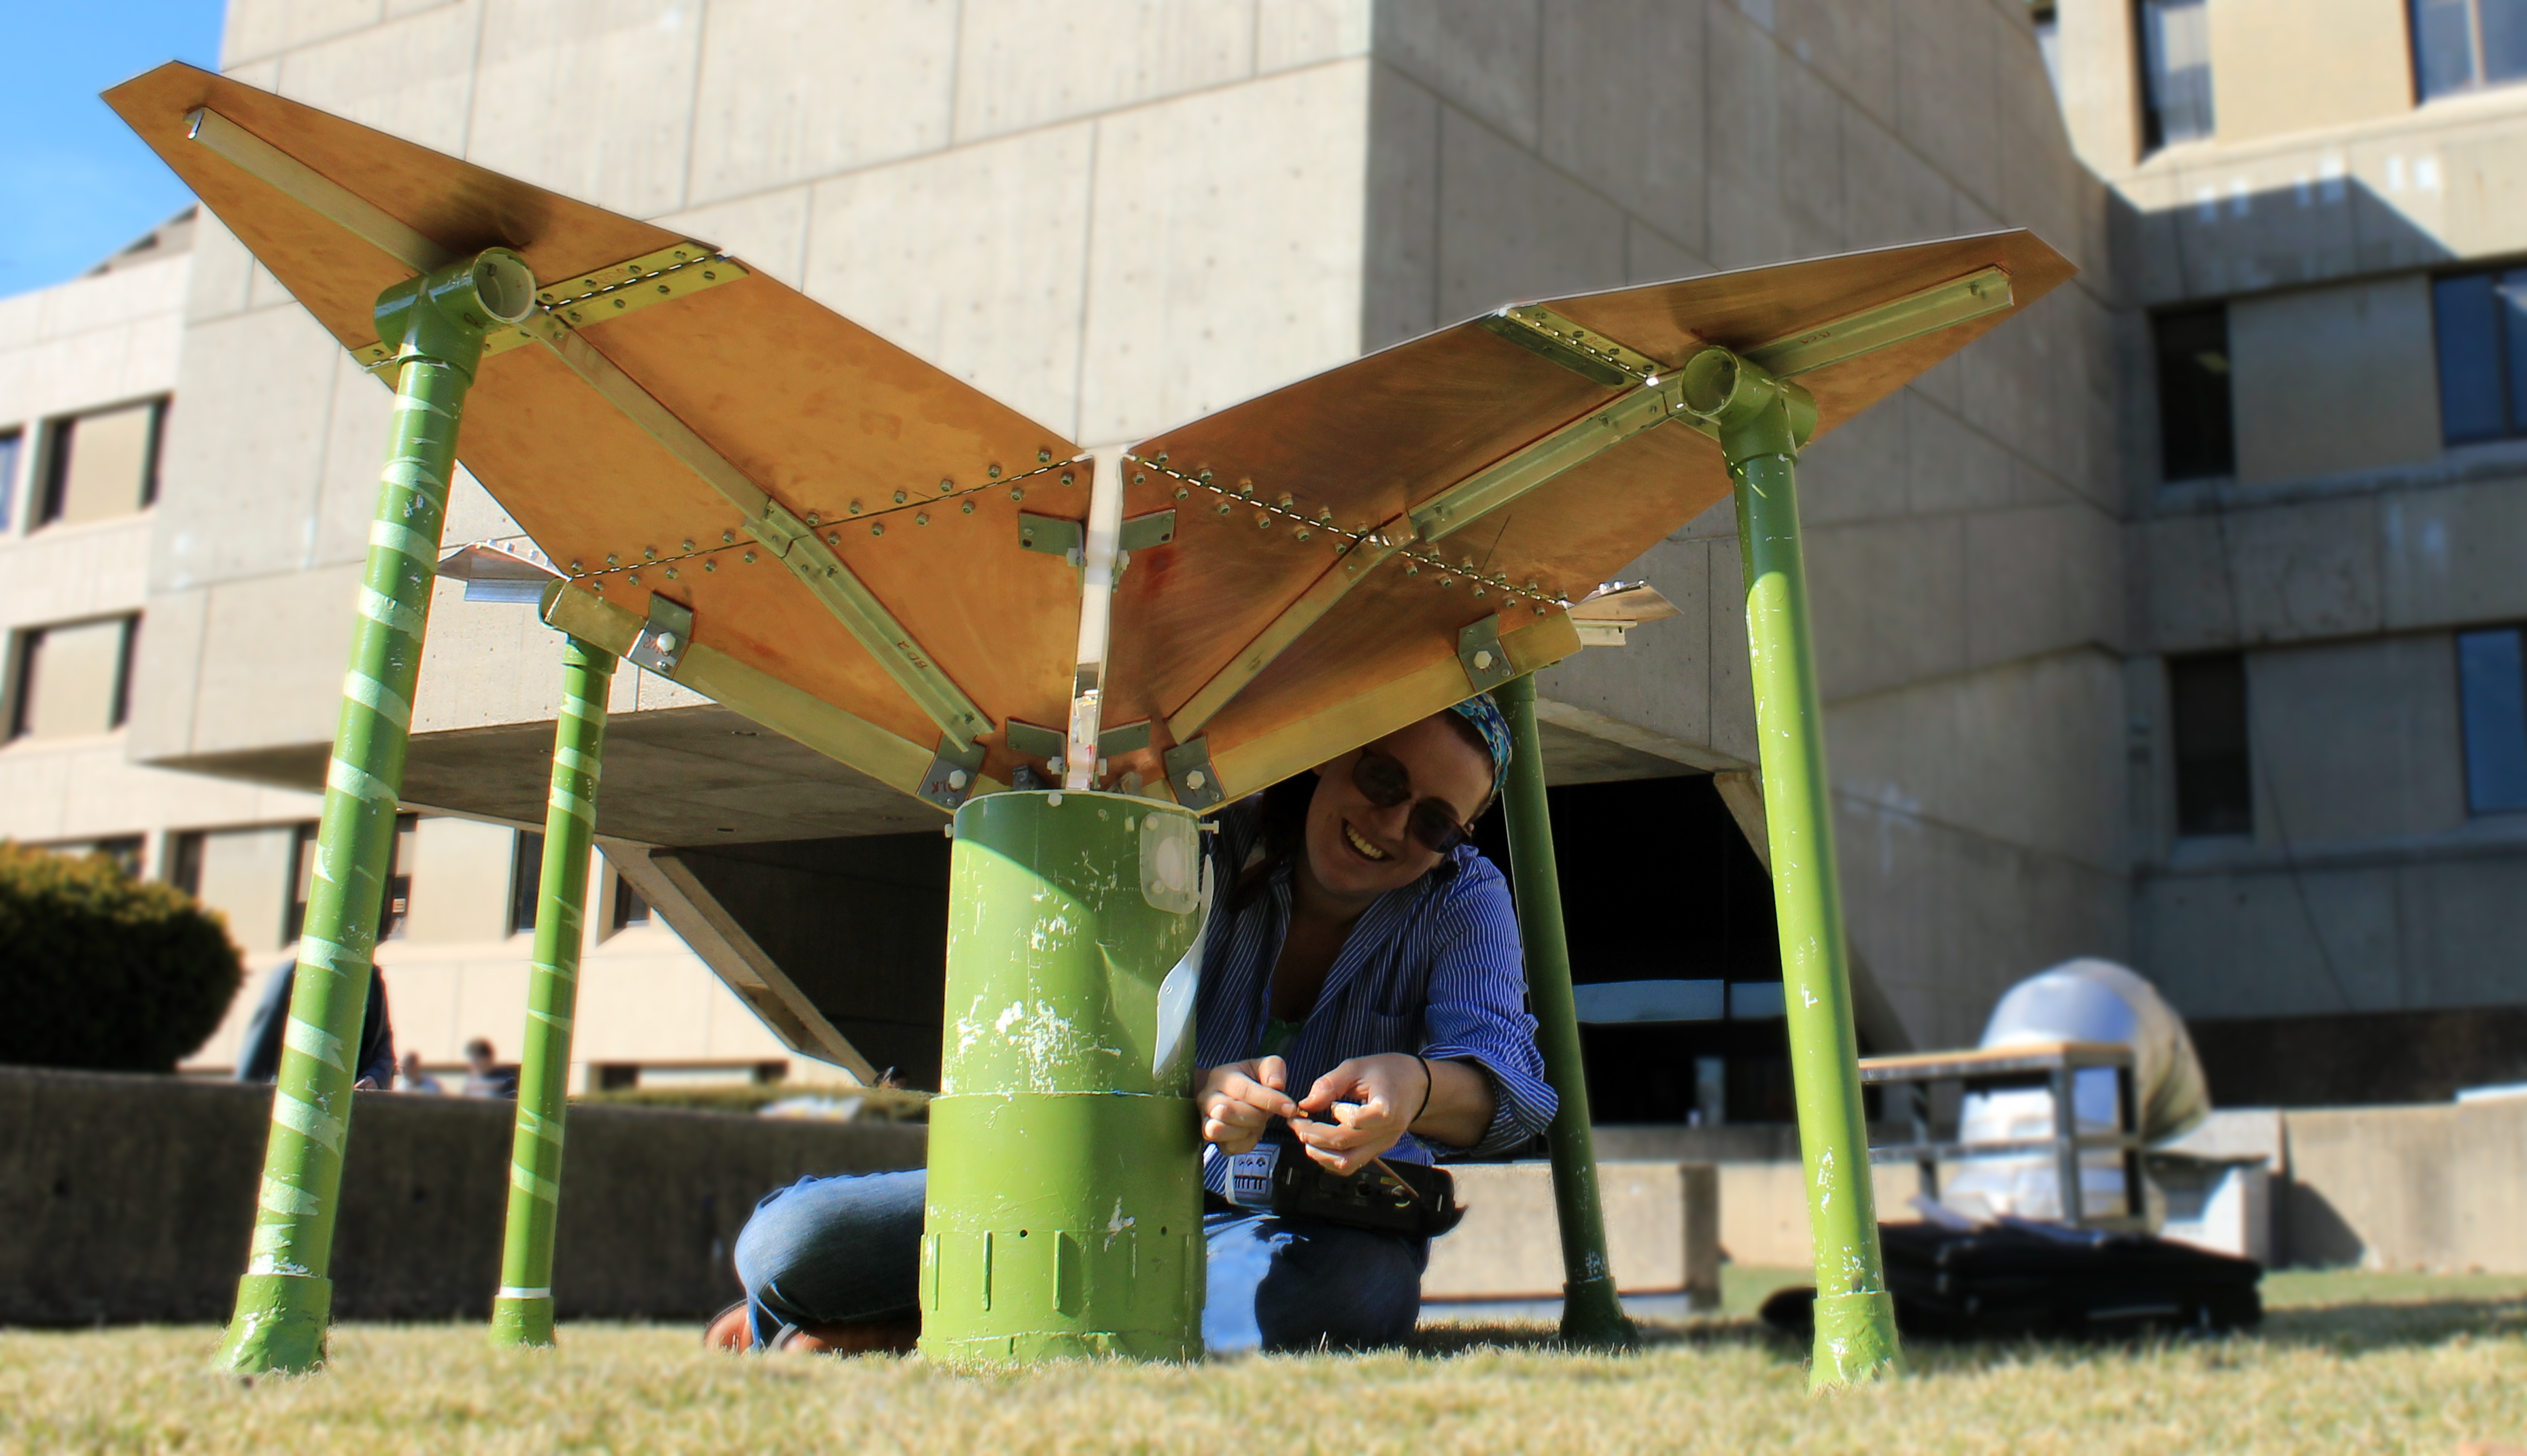
\includegraphics[width=0.95\linewidth]{SCIHI_system/figures/HIbiscus_100mhz.jpg}
\caption{New HIbiscus antenna scaled for $100 MHz$ as set up on the lawn at CMU while its S-parameters were measured. }
\label{Fig:hibiscus_100}
\end{center}
\end{figure}

\subsubsection{Antenna Upgrades} \label{Sec:HIant_upgrade}

Deployment of the SCI-HI system in June 2013 demonstrated that the HIbiscus antenna could use some improvements prior to future deployments. The first and most significant change was the addition of a second antenna scaled to have a center frequency of $100 MHz$. By having both scales ($70 MHz$ and $100 MHz$), data can now be collected over a wider range of frequencies. In addition, the overlap region where both antennas work well ($\sim 85-95 MHz$) provides a cross check for the signal. This cross check will help us to make sure that any spectral structure measured is not coming from the antenna. 

\begin{figure}[htb]
\centering
\begin{minipage}[b]{0.33\textwidth}
\centering
\includegraphics[width=0.95\linewidth]{SCIHI_system/figures/HIbiscus_petals.jpg}
\caption{HIbiscus petals with hinged joints.}
\label{Fig:hibiscus_petal}
\end{minipage}%
\begin{minipage}[b]{0.02\textwidth}
\hspace{1cm}
\end{minipage}%
\begin{minipage}[b]{0.61\textwidth}
\centering
\includegraphics[width=0.95\linewidth]{SCIHI_system/figures/HIbiscus_folded_70mhz.jpg}
\caption{HIbiscus petals folded up in preparation for packing.}
\label{Fig:hibiscus_fold}
\end{minipage}
\end{figure}

We built a new $70 MHz$ HIbiscus antenna (see Figure \ref{Fig:hibiscus_70}) as well as the $100 MHz$ HIbiscus antenna (see Figure \ref{Fig:hibiscus_100}) based on the same simulated antenna design as the original HIbiscus antenna. However, our deployment helped us to identify areas of improvement to the mechanical design of the antenna. These changes are intended to make assembly and travel easier. 

First, we replaced the brass flanges that had to be screwed together to assemble each petal with hinged joints (made out of piano hinge) that do not have to be disassembled and reassembled (see Figure \ref{Fig:hibiscus_petal}). Figure \ref{Fig:hibiscus_fold} shows two of these petals when they are folded and stacked prior to being placed inside a bag for travel. 

Second, we modified the support PVC pipes so that we simply add an extension to the middle of the pipe to adjust the height for the $70 MHz$ HIbiscus antenna compared to the $100 MHz$ antenna. Therefore, adding the $100 MHz$ antenna to the experiment only requires one additional bag beyond the three required to transport the $70 MHz$ antenna. 

\begin{figure}[htb]
\begin{center}
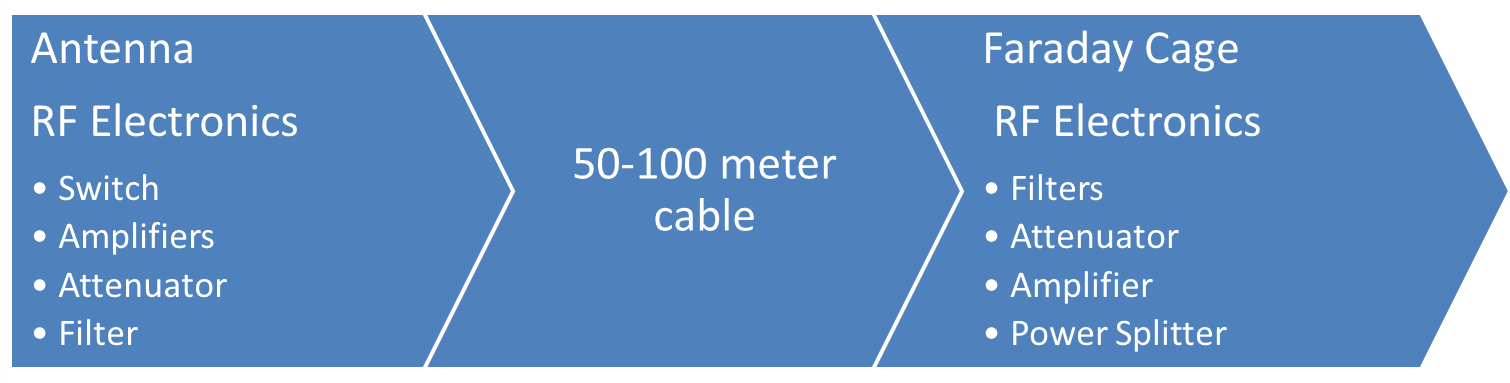
\includegraphics[width=0.9\linewidth]{SCIHI_system/figures/rf_electronics_block_diagram.png}
\caption{Block diagram of the RF Electronics for the SCI-HI instrument.}
\label{Fig:RF_block_diagram}
\end{center}
\end{figure}

\begin{figure}[htb]
\begin{center}
%\centering
%\begin{minipage}[b]{0.47\textwidth}
%\centering

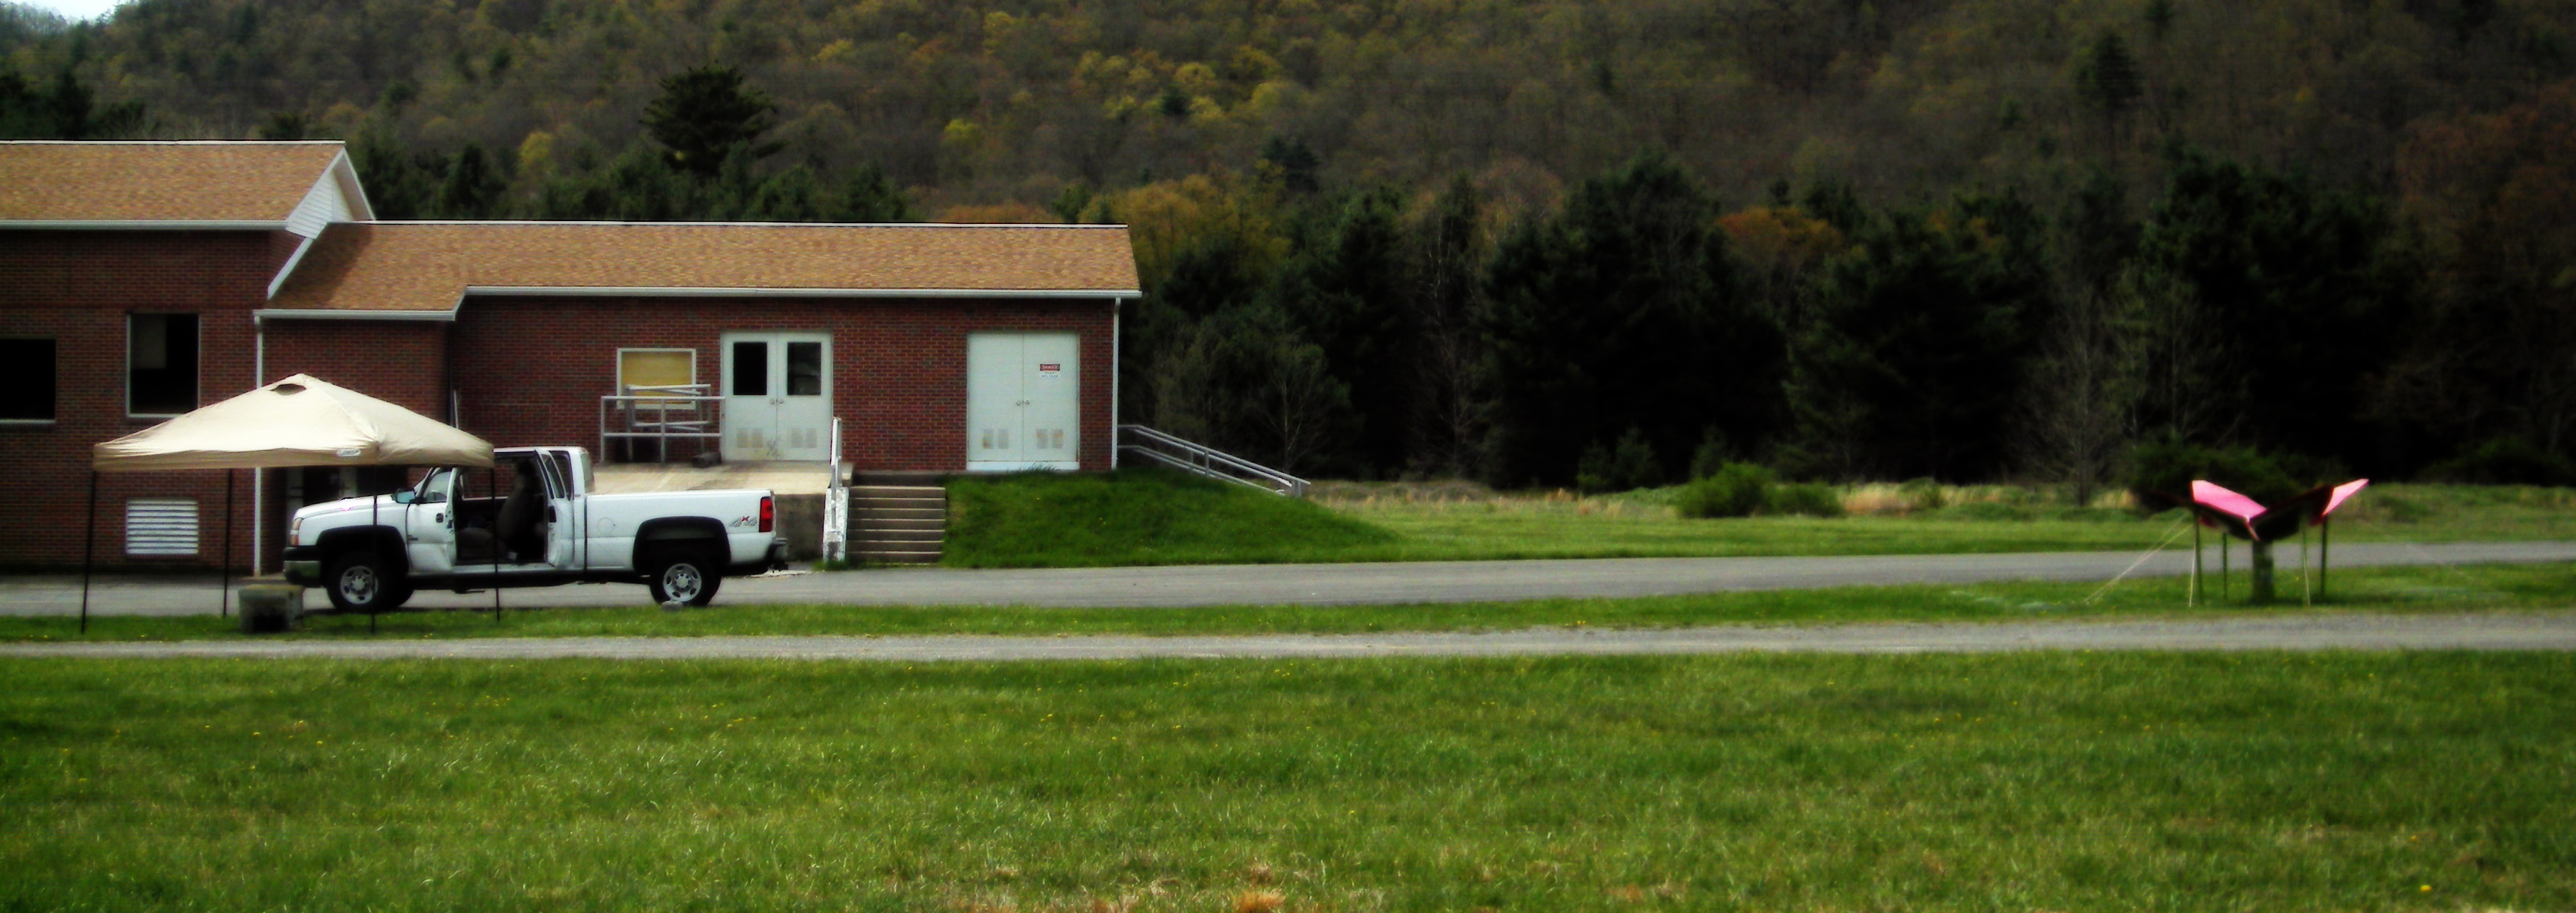
\includegraphics[width=0.95\linewidth]{SCIHI_system/figures/SCIHI_gbt_sys.jpg}
\caption{SCI-HI system with HIbiscus antenna set up on site at Green Bank in May 2013.}
\label{Fig:sys_gbt}

\end{center}
\end{figure}

%\end{minipage}%
%\begin{minipage}[b]{0.02\textwidth}
%\hspace{1cm}
%\end{minipage}%
%\begin{minipage}[b]{0.47\textwidth}
%\centering

\begin{figure}[htb]
\begin{center}
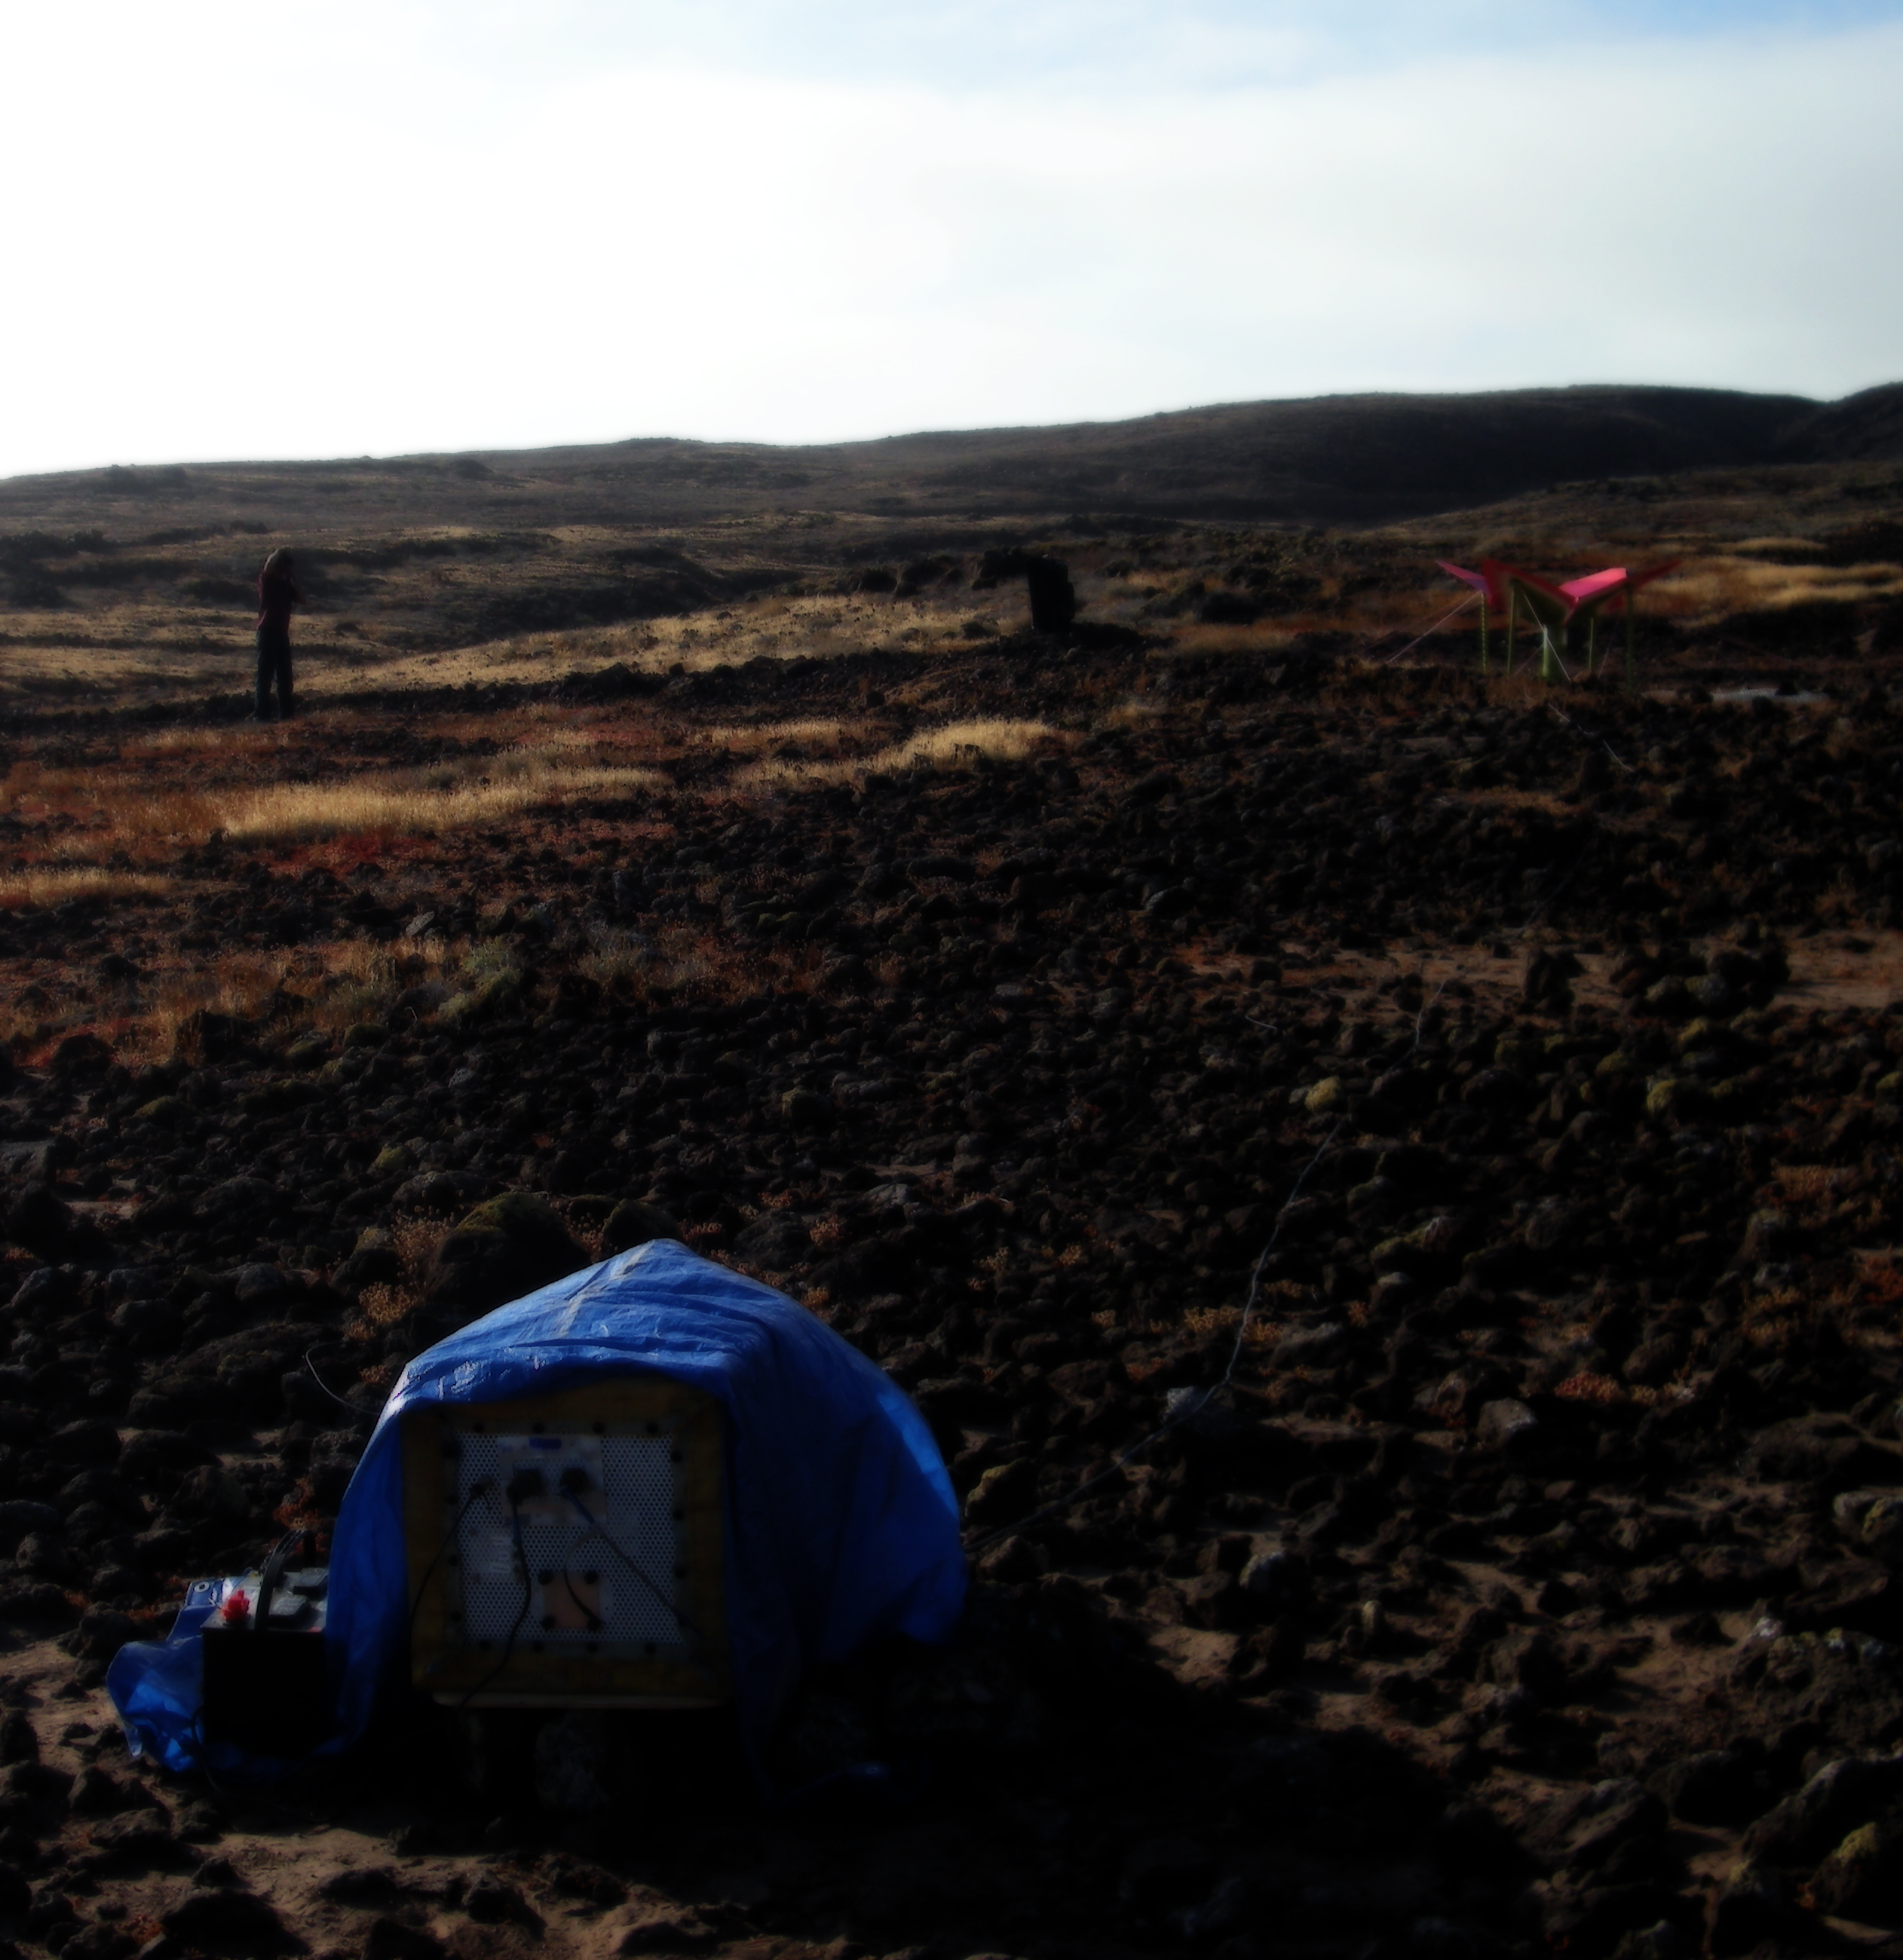
\includegraphics[width=0.85\linewidth]{SCIHI_system/figures/SCIHI_guad_sys.jpg}
\caption{SCI-HI system with HIbiscus antenna set up on site at Isla Guadalupe in June 2013}
\label{Fig:sys_guad}
%\end{minipage}

\end{center}
\end{figure}



\section{RF Electronics}

Once the signal from the sky has been collected by the antenna, it has to be transmitted to the data processing system in a form that the system is capable of processing. Transmission happens along a chain of radio frequency (RF) electronics. 


\subsection{RF Electronics Chain Overview}

For the SCI-HI system, the RF electronics chain components are a switch, amplifiers, high and low pass filters, attenuators and a power splitter (along with the attendant cabling). Each of these components serves a specific purpose in the system. 

We divide the RF electronics chain into two sections based upon physical location, see Figure \ref{Fig:RF_block_diagram}. The first section is the antenna electronics, which sit as close to the antenna terminal as physically possible. The second section is the Faraday Cage electronics, which sit next to the data processing system within a Faraday Cage. Between the two sections is a long signal cable ($\sim50-100 m$), allowing the antenna and data processing system to be placed far enough apart that the transmission of self-generated noise from the data processor is minimized (see Figures \ref{Fig:sys_gbt} and \ref{Fig:sys_guad}).

\begin{figure}[htb]
\centering
\begin{minipage}[b]{0.47\textwidth}
\centering
\includegraphics[width=0.95\linewidth]{SCIHI_system/figures/trombone_sys_switch.jpg}
\caption{Trombone antenna set-up with calibration switch mounted directly below the antenna.}
\label{Fig:trombone_switch}
\end{minipage}%
\begin{minipage}[b]{0.02\textwidth}
\hspace{1cm}
\end{minipage}%
\begin{minipage}[b]{0.47\textwidth}
\centering
\includegraphics[width=0.95\linewidth]{SCIHI_system/figures/SCIHI_rf_ant_lower.jpg}
\caption{RF electronics box at the base of the Trombone antenna with second stage amplifier and filters.}
\label{Fig:trombone_base}
\end{minipage}
\end{figure}

\begin{figure}[htb]
\begin{center}
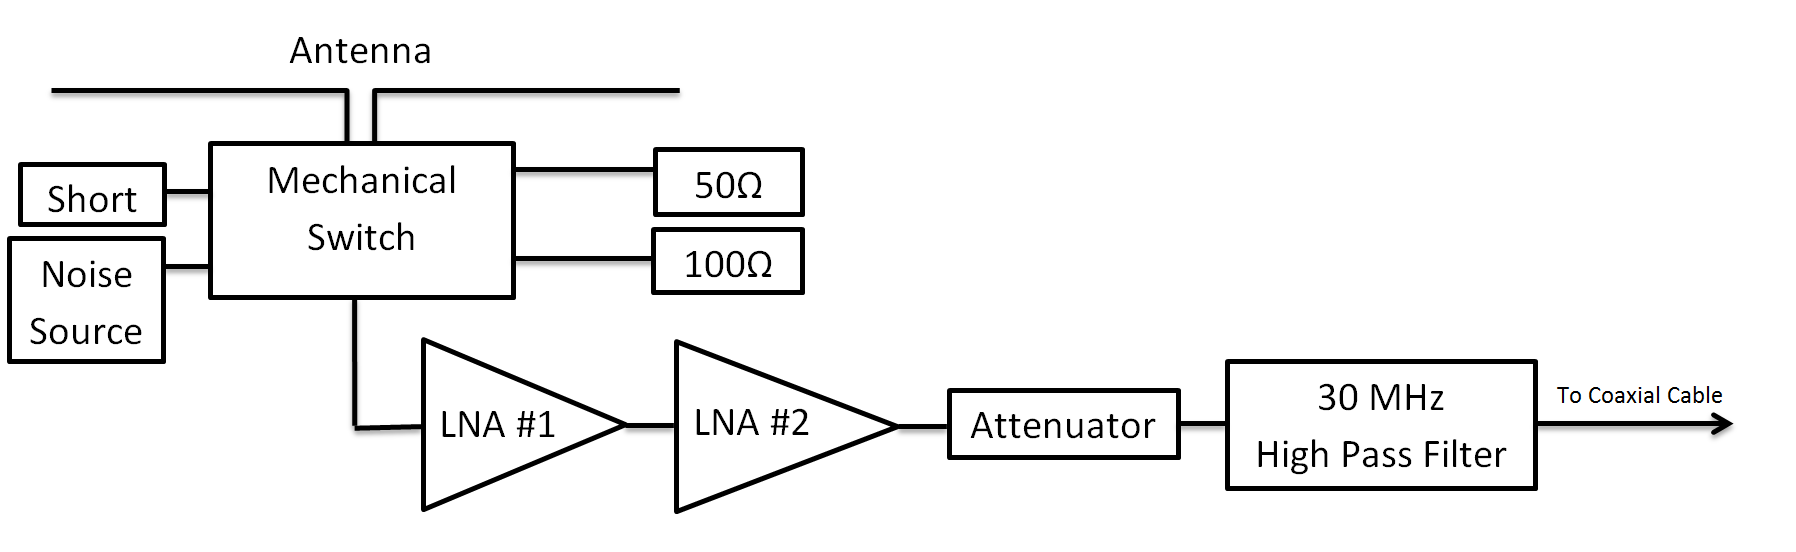
\includegraphics[width=0.9\linewidth]{SCIHI_system/figures/antenna_rf_block_diagram.png}
\caption{Block diagram of the RF Electronics located at the base of the antenna.}
\label{Fig:antenna_RF_block_diagram}
\end{center}
\end{figure}


\subsection{Antenna Electronics}

The antenna electronics are a calibration switch with known signal sources on some of the terminals, and two stages of amplification. In some versions of the electronics system, at least one of the RF filters was also placed at the antenna end of the system. The layout of the antenna electronics is shown in Figure \ref{Fig:antenna_RF_block_diagram}. 

\subsubsection{Calibration Switch} \label{Sec:switch}

Because the SCI-HI system has a single antenna with a relatively large beam, calibrating the data from the antenna can be difficult. One way to do this calibration is to use a noise source of known temperature whose signal is sent through the same RF chain as the antenna data (see Chapter \ref{Ch:Data}). 

In order to facilitate this calibration, a switch was placed at the terminal of the antenna. By making the antenna one of the inputs of the switch and matching one or more known temperature sources to the other switch inputs, data can be collected for all inputs with the same RF chain. 

We used a 6 input electromechanical switch purchased on eBay (Narda SEM066 SP6T\footnote{\url{http://www.nardamicrowave.com/east/index.php}}) for the system. One input to the switch was connected directly to the antenna (see Figures \ref{Fig:trombone_switch} and \ref{Fig:rf_ant_mount}). The other inputs are a short terminator, a $50 \Omega$ load terminator, a $100 \Omega$ load terminator, and an artificial noise source of known power. One input was left open. 

Switching between inputs is controlled through a cable from the Faraday Cage that carries both the power for the antenna electronics and the control signal. In addition, the artificial noise source is turned off when that input is not enabled (to avoid noise bleeding into the antenna). We also built a manual switch control box that can be hooked up to the switch for testing and runs off a small battery pack. 

\begin{figure}[htb]
\centering
\begin{minipage}[b]{0.47\textwidth}
\centering
\includegraphics[width=0.95\linewidth]{SCIHI_system/figures/SCIHI_rf_ant_box.jpg}
\caption{New lucite box containing all the antenna RF electronics.}
\label{Fig:rf_ant_box}
\end{minipage}%
\begin{minipage}[b]{0.02\textwidth}
\hspace{1cm}
\end{minipage}%
\begin{minipage}[b]{0.47\textwidth}
\centering
\includegraphics[width=0.95\linewidth]{SCIHI_system/figures/SCIHI_rf_ant_box_mount.jpg}
\caption{RF electronics box attached to one of the HIbiscus antenna center mounts.}
\label{Fig:rf_ant_mount}
\end{minipage}
\end{figure}

\subsubsection{Amplifiers} \label{Sec:Amp}

Immediatelly following the switch in the RF chain is the first stage low noise amplifier (LNA). This amplifier should have a low noise figure, as amplifier noise will be added to the incoming RF signal before amplification. In addition, the LNA should have an impedance that is well matched to the antenna. Matching is necessary for signals from the antenna to be transmitted by the LNA instead of being reflected back out the antenna. 

\paragraph{Impedance} 

Impedance ($Z$) is the complex ratio ($Z = V/I$) of a circuit element. It is measured using the circuit element reflectivity ($S11$) relative to a reference impedance, which is usually $50 \Omega$ \cite{stutzman1981}.

\begin{equation}\label{Eq:Imp_calc}
Z(\nu) = R(\nu)+ i X(\nu) 
\end{equation}
\begin{equation}
R(\nu) = \frac{50 (1-|S11(\nu)|^2)}{(1-\Re(S11(\nu)))^2 + \Im(S11(\nu))} 
\end{equation}
\begin{equation}
X(\nu) = \frac{100 \Im(S11(\nu))}{(1-\Re(S11(\nu)))^2 + \Im(S11(\nu))} 
\end{equation}

\paragraph{Impedance Matching}

The presence of reflectivity means that not all of the signal sent down a circuit will reach its final destination. Some of the signal will instead be reflected back toward its source. The exact magnitude of this reflectivity at each interface between circuit elements is set by the match between the impedances of the two elements. 

\paragraph{Transmission Efficiency ($\eta$)}

If $Z_{Source} = Z^*_{Load}$, then all of the signal is transmitted. Otherwise, some of the signal power is reflected. The fraction of signal power that is transmitted is called the transmission efficiency ($\eta$). Equation \ref{Eq:eta} gives the relationship between the impedances of two circuit elements and the percentage of signal which is transmitted. 

\begin{equation} \label{Eq:eta}
\eta (\nu) = \sqrt{\frac{4 |R_{S}*R_{L}|}{(R_{S}+R_{L})^2+(X_{S}+X_{L})^2}}
\end{equation}

\paragraph{Cable Delay}

In our case the interface of interest is the one between the antenna and the first stage amplifier, $Z_S = Z_{ant}$ and $Z_L = Z_{amp}$. However, the antenna impedance as seen by the LNA will be modified by the cable between the antenna and LNA. 

This modification will not change the magnitude of $Z$, but will affect its complex phase as $Z_{mod} = |Z_{orig}| e^{2 \pi i \tau \nu }$. The magnitude of $\tau$ is set by the length of the cable and its propogation constant ($C_{cable}$), $\tau = l_{cable} C_{cable}$. The propogation constant $C_{cable}$ is based upon the cable's index of refraction n and has a value of $C_{cable} \approx 0.125$ ns/inch for coaxial cable. 

\begin{figure}[htb]
\centering
\begin{minipage}[b]{0.47\textwidth}
\centering
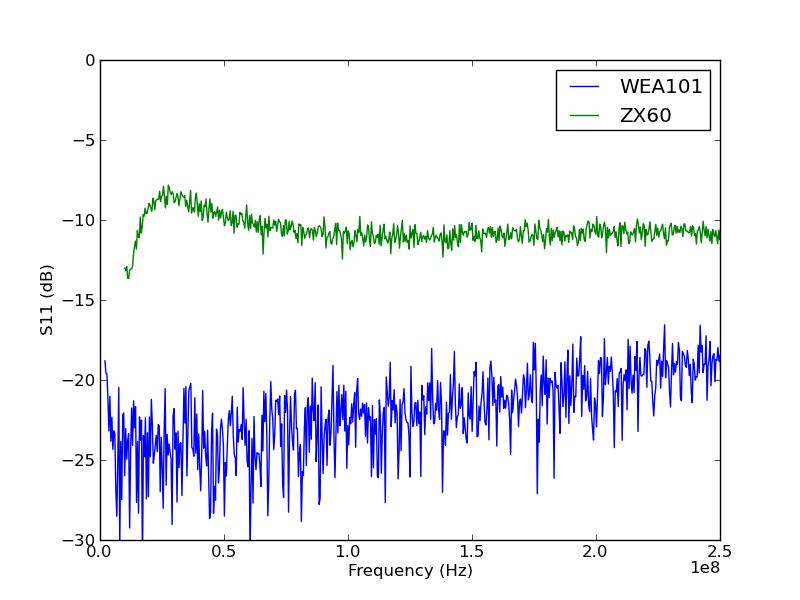
\includegraphics[width=0.95\linewidth]{SCIHI_system/figures/amp_S11_dB.png}
\caption{Amplifier reflectivity ($S11$) in dB for the two amplifiers used in the SCI-HI system.}
\label{Fig:amp_comp_dB}
\end{minipage}%
\begin{minipage}[b]{0.02\textwidth}
\hspace{1cm}
\end{minipage}%
\begin{minipage}[b]{0.47\textwidth}
\centering
\includegraphics[width=0.95\linewidth]{SCIHI_system/figures/amp_S11_Smith.png}
\caption{Smith chart of the reflectivity of the two amplifiers used in the SCI-HI system. Data is shown for $20-250 MHz$. }
\label{Fig:amp_comp_Smith}
\end{minipage}
\end{figure}

\begin{figure}[htb]
\begin{center}
\includegraphics[width=0.9\linewidth]{SCIHI_system/figures/amp_Gain_dB.png}
\caption{Amplifier gain ($S21$) in dB for the two amplifiers used in the SCI-HI system. }
\label{Fig:amp_gain}
\end{center}
\end{figure}

\paragraph{Amplifier Selection}

In order to minimize loss due to impedance mismatch, we want an amplifier whose impedance is the complex conjugate of the antenna impedance. I tested a number of LNAs to find one whose impedance was matched to our antenna over the entire frequency band of interest for SCI-HI. 

I started with a Minicircuits\footnote{\url{http://www.minicircuits.com}} packaged amplifier ($ZX60 - 33 LN - S+$) with a low noise figure ($\sim 1$ dB) and wide bandwidth. Unfortunately this amplifier's impedance was a poor match for the antenna, but we were able to make use of the amplifier later in the RF chain (see Section \ref{Sec:fcage_elec}). 

Next, I tried to use the Avago Technologies\footnote{\url{http://www.avagotech.com/}} amplifier chip ($MGA-633P8$), which we had previously used for higher frequency applications. The benefit of using a chip versus a pre-packaged amplifier was that I could modify the circuit around the chip to tune the impedance to match the antenna. However, I was unable to tune the chip circuit to simultaneously get the desired impedance and maintain the amplifier gain in our frequency band. This was primarily due to the fact that the chip was designed for higher frequencies around $700 MHz$. 

Therefore, I went hunting again for a packaged amplifier that fit my specific impedance needs. Richardson RFPD\footnote{\url{http://www.richardsonrfpd.com/}} has a packaged low noise amplifier ($WEA-101$), whose impedance was a better match to the antenna than the Minicircuits amplifier. Figures \ref{Fig:amp_gain}, \ref{Fig:amp_comp_dB}, and \ref{Fig:amp_comp_Smith} show the $S11$ (reflectivity) and $S21$ (gain) of the two amplifiers for the SCI-HI frequency band. 

Unlike the $ZX60$ amplifier, the $WEA101$ amplifier has an almost entirely real impedance, which is nearly constant over our frequency band. It also has a very low reflectivity. This makes the $WEA101$ amplifier an excellent choice as a first stage amplifier. 

\begin{figure}[htb]
\begin{center}
\includegraphics[width=0.9\linewidth]{SCIHI_system/figures/antenna_rf_cable_reflections.png}
\caption{Large scale oscillation in the short calibration data due to a cable between the first and second stage amplifiers. Blue is the data with the original 1 meter cable, green is the data with a 2 meter cable, and red is the data with the amplifiers right next to each other.}
\label{Fig:amp_reflect}
\end{center}
\end{figure}

\paragraph{Multi-Stage Amplification}

Because the $\sim 50-100 m$ signal cable will attenuate signals travelling down its length, a second stage amplifier was added to the system to increase the gain of the signal. Initially the second stage amplifier was placed at the base of antenna (see Figure \ref{Fig:trombone_base}). However, this placement resulted in reflections in the signal whose period corresponded to the cable length between the two amplifiers. This is shown in Figure \ref{Fig:amp_reflect}. We confirmed that the cable between the amplifiers was the source of the oscillation by replacing the cable with one twice as long. When we did this the period of the oscillation was cut in half, as shown in Figure \ref{Fig:amp_reflect}. 

Therefore, we moved the second stage amplifier to a position immediately following the first stage amplifier (see Figure \ref{Fig:rf_ant_box}). This removed the cable reflections, as shown in Figure \ref{Fig:amp_reflect}. The total gain of the amplifiers was $\sim 50$ dB over the entire frequency band. Both amplifiers use DC power supplied by the same power cable as the switch. As different levels of DC voltage are needed for the individual electronic components, voltage regulation circuits are also included in the antenna electronics housing. 

\begin{figure}[htb]
\begin{center}
\includegraphics[width=0.9\linewidth]{SCIHI_system/figures/antenna_rf_power_block_diagram.png}
\caption{Wiring block diagram for the antenna RF electronics.}
\label{Fig:ant_RF_pow_block_diagram}
\end{center}
\end{figure}

\subsubsection{Antenna Power and Switch Control} \label{Sec:ant_pow}

Power and switch control signals are sent along a cable that runs parallel to the signal cable from the Faraday Cage to the base of the antenna. This cable has an Amphenol\footnote{\url{http://www.amphenol.com/}} 23 pin circular mil spec connectors on each end, of which 7 pins are used. One pin is ground, one is DC power, and the other five are control signals for each of the switch inputs. 

Power to each of the antenna RF components is supplied following the diagram in Figure \ref{Fig:ant_RF_pow_block_diagram}. The two amplifiers use 5 V regulated power, while the noise source has 15 V regulated power which is only supplied when the noise source is being measured through the switch. Control of the noise source power input is handled by a Teledyne\footnote{\url{http://www.teledynerelays.com/}} optically isolated relay module. 

In earlier versions of the SCI-HI system, the power from the Faraday Cage was $V< 15$V, so a 9V battery was added to the noise source circuit to supply the additional voltage. This battery was only in use when the noise source was switched on. For the current version of the system, the switch needs $V \geq 18$V. This negates the need for a supplemental battery, as the power sent to the antenna electronics will always be $V \geq 15$V.  

\begin{figure}[htb]
\begin{center}
\includegraphics[width=0.9\linewidth]{SCIHI_system/figures/faraday_cage_rf_block_diagram.png}
\caption{Block diagram of the RF Electronics located inside the Faraday Cage.}
\label{Fig:fcage_RF_block_diagram}
\end{center}
\end{figure}


\subsection{Faraday Cage Electronics}

Once the signal has travelled down the long cable from the antenna, there are a few electronic stages that it must pass through prior to entering the data processing system. A third stage amplifier is needed to compensate for the attenuation caused by the long cable, filters are needed to keep signals from outside the frequency band of interest from overloading the data processing system or leaking into the band, and a signal power splitter used to achieve the necessary data sampling rate. The layout of these electronics is shown in Figure \ref{Fig:fcage_RF_block_diagram}. All of the RF electronics, as well as the data processing system, were placed inside a Faraday Cage designed specifically to accomodate them. 

\subsubsection{RF Filters and Amplification} \label{Sec:fcage_elec}

Once the signal from the antenna entered the Faraday Cage, the first part of the RF chain was a set of filters. These filters were a low pass filter at $200 MHz$ (Minicircuits $SLP-200+$) and a high pass filter at $30 MHz$ (Minicircuits $SHP-25+$). The low pass filter was placed to prevent signals from higher frequencies ($\geq 200 MHz$) from aliasing into the frequency range where we were observing. The high pass filter was placed to prevent signals from the shortwave band and below overloading the sampling system, which could affect the overall system gain or create spurious signals in the observing band. 

After the signal has passed through the long cable and the filters, it is necessary to add another level of amplification to the system. This final stage of amplification is to bring the signal levels to a point where they can be clearly distinguished from system noise by the data processing system and adds $\sim25$ dB of gain. The amplifier used here is a Minicircuits amplifier ($ZX60-33LN-S+$), which is supplied with 5V regulated power from the DC source. 

\subsubsection{RF Signal Splitting} \label{Sec:hard_split}

The Analog-to-Digital Conversion (ADC) card used in the data processing system is limited to a 250 MSamples-per-sec sampling rate, but the desired bandwidth of the system is over $125 MHz$. In order to expand the operating range of the ADC, a hardware $''$trick$''$ is used.

The signal from the antenna is split into two identical signals with a Minicircuits power splitter ($ZFSC-2-1$). Both signals are then sent into the ADC through two of the input ports. However, the lengths of the cables placed between the two outputs of the splitter and the two input ports of the ADC are slightly different. The difference ($\sim 50 \; cm$) is exactly calculated so that a sample taken from one input port is has been delayed by 2 ns compared to the other input port. If the signals from both ports are combined, the data has now been sampled at 500 MSamples-per-sec. This interleaved sampling is common in high bandwidth ADC systems. 

\begin{figure}[htb]
\begin{center}
\includegraphics[width=0.9\linewidth]{SCIHI_system/figures/fcage_rf_power_block_diagram.png}
\caption{Wiring block diagram for the Faraday Cage RF electronics.}
\label{Fig:fcage_RF_pow_block_diagram}
\end{center}
\end{figure}

\subsubsection{Faraday Cage RF Electronics Power Supply}

Power is supplied to the RF electronics inside the Faraday Cage and at the base of the antenna through a common source (DC battery or AC generator, see Section \ref{Sec:sys_power}). Assuming that the Faraday Cage input power is AC, the power is distributed as shown in Figure \ref{Fig:fcage_RF_pow_block_diagram}. Some of the power travels to the antenna RF electronics via the system power/control cable that runs parallel to signal cable. This power is discussed in full detail in Section \ref{Sec:ant_pow}. 

\begin{figure}[htb]
\begin{center}
\includegraphics[width=0.9\linewidth]{SCIHI_system/figures/fcage_pp_con_circuit_diagram.png}
\caption{Circuit diagram for the parallel port switch control circuit.}
\label{Fig:fcage_ppcon_block_diagram}
\end{center}
\end{figure}

\subsubsection{Switch Control Circuit}

In order to get the control signal for the switch from the data processing system into the RF chain, a small circuit is necessary. This circuit, shown in Figure \ref{Fig:fcage_ppcon_block_diagram}, uses a transistor array chip ($ULN2003A$) to change the switch control voltages to the necessary levels based on the parallel port output signals. The control circuit lives inside the Faraday Cage with the computer (see Figure \ref{Fig:fcage_RF_pow_block_diagram}). 

\begin{figure}[htb]
\centering
\begin{minipage}[b]{0.37\textwidth}
\centering
\includegraphics[width=0.95\linewidth]{SCIHI_system/figures/SCIHI_fcage_old.jpg}
\caption{Faraday Cage around data processing system as set-up in October 2012.}
\label{Fig:fcage_old}
\end{minipage}%
\begin{minipage}[b]{0.02\textwidth}
\hspace{1cm}
\end{minipage}%
\begin{minipage}[b]{0.61\textwidth}
\centering
\includegraphics[width=0.95\linewidth]{SCIHI_system/figures/SCIHI_filter.jpg}
\caption{System power and control signal filter box for one of the Faraday Cages.}
\label{Fig:fcage_filter}
\end{minipage}
\end{figure}

\subsection{SCI-HI Faraday Cage and System Power}

\subsubsection{Farday Cage Design}

The design of the Faraday Cage for the SCI-HI system was inspired by the dual requirements of space and portability. Because the wavelengths being studied with the system are $\lambda \geq 1$ meters, metal mesh is used in place of solid metal for the sides of the cage. This mesh is considerably lighter than solid metal, but does not hold its structure. So I came up with a design that uses a metal mesh bag with a PVC pipe framework placed inside to hold its shape (see Figure \ref{Fig:fcage_old}). The mesh bag folds up like a paper bag and the PVC framework can be disassembled and packed into a suitcase. 

Access to the Faraday Cage is supplied through the front panel, which attaches to the rest of the bag through a set of metal snaps spaced less than $20 \; cm$ apart. This front panel includes access ports for the signal cable, as well as the power and switch control cable. Multiple versions of the Faraday Cage were constructed, all of which used the mesh bag concept (see Figures \ref{Fig:fcage_old}, \ref{Fig:fcage_int}, and \ref{Fig:fcage_new}). 

\begin{figure}[htb]
\centering
\begin{minipage}[b]{0.46\textwidth}
\centering
\includegraphics[width=0.95\linewidth]{SCIHI_system/figures/SCIHI_fcage_int.jpg}
\caption{Faraday Cage around the data processing system as set-up in June 2013.}
\label{Fig:fcage_int}
\end{minipage}%
\begin{minipage}[b]{0.02\textwidth}
\hspace{1cm}
\end{minipage}%
\begin{minipage}[b]{0.52\textwidth}
\centering
\includegraphics[width=0.95\linewidth]{SCIHI_system/figures/SCIHI_fcage_new.jpg}
\caption{Faraday Cage with double shielding around data processing system, currently under development.}
\label{Fig:fcage_new}
\end{minipage}
\end{figure}

\subsubsection{Faraday Cage Power Filters}

Because the power and switch control cable carries DC power out to the antenna electronics, it needs to be filtered to keep RF signals from using the cable to escape the Faraday Cage. To accomplish this, a set of filter boxes are placed in the DC power and switch control signal lines. These filter boxes (see Figure \ref{Fig:fcage_filter}) are low pass capacitive filters with over 40 dB of attenuation above $40 MHz$. Two stages of filtering are included to ensure that there is no signal transmission through the DC power lines. 

Initially the power supply battery lived inside the Faraday Cage (see Figure \ref{Fig:fcage_old}). Eventually, it was moved outside the cage to simplify battery swapping (see Section \ref{Sec:sys_power}). At this point filters also had to be used between the battery and the electronics inside the cage. The same filters used for the DC power and switch control cable were also used for the battery cable. This ensures that RF signals don't use the battery cable to transmit outside the Faraday Cage.  

\subsubsection{System Power Selection} \label{Sec:sys_power}

The entire system was powered using deep-cycle automotive batteries. These batteries supplied 12 V unregulated power, which was used by both the data processing system and the RF electronics. A fully charged battery could power the entire system for $\sim12-15$ hours. 

Charging batteries was a big part of the support process for the SCI-HI system. Keeping the system running continually required at least 3 batteries with regular access to a battery charger and transport between the SCI-HI site and the battery charging location 2-3 times a day. In addition, recent upgrades to the SCI-HI system include components that need DC voltages larger than 12 V. Therefore, alternative power sources have been investigated.

One alternative power sources is a small portable gasoline or diesel generator. Using this generator would cut down on the number of site visits required, as the generator would run constantly with only occasional stops to top off the fuel. The generator would also allow us to supply larger DC voltages as needed. 

However, using a generator leads to a new source of RF noise (particularly a gasoline generator with spark plugs). Placing the generator inside its own Faraday Cage should attenuate this noise, but it is a factor that must be accounted for in selecting a power source. 


\section{Data Processing System}


\subsection{Data Processing Pathway}

As discussed in Section \ref{Sec:hard_split}, signals from the electronics enter the data processing system via two ports of an Analog-to-Digital Conversion (ADC) card. For the SCI-HI system, we used a GE PCIe digitizer board ($ICS1650$). Data is collected for one second of integration, with the interleaving strategy producing 500 MSamples-per-sec of data. 

Storing the entire dataset for each second would require a great deal of space. Instead, a Fast Fourier Transform (FFT) is performed on the sampled time streams, then the power signals are averaged. The averaged power spectrum produced by the FFT is much smaller than the raw data. This spectrum is stored by the system, after which the process is repeated for another second of data. 

Because of the limited bandwidth from the ADC to the rest of the system, sampling of a new data stream requires the FFT of the previous data stream to be complete. This means that the system is less than 100\% efficient, it takes longer than 1 second to record the power spectrum of 1 second of data. Initially the FFT calculation was quite time consuming ($\sim 30-60$ seconds), but improvements to the software and hardware by Jose-Miguel have decreased this calculation time to $\sim 2$ seconds. This means that the system has a duty cycle of $\sim30$\%. 

All of the frequency spectrum data is stored locally on the hard drive of the processing system. The relatively small data volume ($\sim 2$ GB per day) means that data transfer can be done using small USB drives. During deployment, data was removed from the hard drive 2-3 times a day and stored locally on multiple laptop computers and external hard drives before being uploaded to a server upon return to $''$civilization$''$ (aka the lab). 

\begin{figure}[htb]
\centering
\begin{minipage}[b]{0.54\textwidth}
\centering
\includegraphics[width=0.95\linewidth]{SCIHI_system/figures/SCIHI_UI_Screen.jpg}
\caption{User interface layout for the SCI-HI system. Data shown is zeros because the system was not hooked up to the antenna at the time the image was taken.}
\label{Fig:GUI}
\end{minipage}%
\begin{minipage}[b]{0.02\textwidth}
\hspace{1cm}
\end{minipage}%
\begin{minipage}[b]{0.43\textwidth}
\centering
\includegraphics[width=0.95\linewidth]{SCIHI_system/figures/SCIHI_raspberry_pi.jpg}
\caption{Raspberry Pi system control computer used for diagnostic purposes in the field. }
\label{Fig:raspberry_pi}

\end{minipage}
\end{figure}


\subsection{System Control and User Interface}

In addition to the data processing software, a graphical user interface was designed by Jose-Miguel for diagnostic and control purposes. This interface displays the most recent frequency spectrum collected by the system and lets the user set the current data collection mode (including switch control). The user can choose to either take a single data set with any of the switch positions (Antenna, 50 $\Omega$, Short, Noise Source, 100 $\Omega$), or take continual data with a set number of antenna datasets followed by a single dataset from each of the calibration sources. Figure \ref{Fig:GUI} shows an example screenshot of the user interface. In this screenshot, the data is $\sim0$ because the electronics and antenna are not connected to the system. 

The system default upon start-up is to run in continual data collection mode with the number of antenna iterations per cycle set by the previous data collection run. To lower the power consumption and space requirements of the system, the software can run without a monitor, mouse and keyboard. Instead, the system can be controlled by an external system through an ethernet port. This port is only used during system monitoring, and can be sealed to prevent RF leakage at all other times. 


\subsection{Control Computer}

The data processing system can be monitored using a personal computer (such as a laptop) with an ethernet port. However, an additional diagnostic computer was also developed by Jose-Miguel for the SCI-HI system. This computer is a Raspberry Pi\footnote{www.raspberrypi.org} with a small monitor, mouse and ethernet port, built by Jose-Miguel and shown in Figure \ref{Fig:raspberry_pi}. Using this small computer, we can quickly check that the system is working properly and run simple diagnostics.

\subsection{Power Supply and Consumption}
In order to power the data processing system, a computer power supply had to be selected that matched the system power source (DC battery). Initially, we started with a typical AC computer power supply and a DC to AC inverter that converted the incoming DC power from batteries into AC power that the computer could handle. 

While using an inverter is the simplest solution, it can be very energy inefficient. For example, the 800 W inverter that we have previously used in the field is $\sim70$\% efficient. Additionally, any failure of the inverter can crash the entire system. Therefore, we decided to switch to an entirely DC system by replacing the AC power supply for the computer with a M4-ATX DC power supply. This power supply takes input DC power of 8-30 V and converts it to the DC power that the motherboard and other systems need. 

Utilizing this power supply lowered our power consumption. However, we found that the power supply we selected was not reliable on long time scales. Since most of the DC power supplies on the market are designed for automotive applications, they are designed for reliability when run for short durations on higher battery (voltage) levels. The DC power supplies were particularly unhappy when running on a nearly drained battery, which had a voltage level close to the minimum required voltage for the power supply. We are currently exploring alternatives for the system, as discussed in Section \ref{Sec:sys_power}. 

\begin{figure}[htb]
\centering
\begin{minipage}[b]{0.52\textwidth}
\centering
\includegraphics[width=0.95\linewidth]{SCIHI_system/figures/SCIHI_comp.jpg}
\caption{Current version of the data processing system assembled inside a Faraday Cage box.}
\label{Fig:new_comp}
\end{minipage}%
\begin{minipage}[b]{0.02\textwidth}
\hspace{1cm}
\end{minipage}%
\begin{minipage}[b]{0.44\textwidth}
\centering
\includegraphics[width=0.95\linewidth]{SCIHI_system/figures/SCIHI_water_cooling_pipe.jpg}
\caption{Copper tubing with brass mounting used for the water cooling system for the data processing machine.}
\label{Fig:water_pipe}
\end{minipage}
\end{figure}


\subsection{System Noise Generation} \label{Sec:sys_noise}

Deployment to Isla Guadalupe in June 2013 indicated that our Faraday Cage design had insufficient attenuation of self-generated RFI from the data processing system. This problem was not identified until deployment at the final site due to masking from external RFI at our testing sites. 

Self-generated RFI was particularly noticeable above $90 MHz$, as can be seen in Figure \ref{Fig:raw_data}. It is also believed to be present in the data at lower frequencies as well. Our data indicated that the strength of the self-generated RFI was correlated with the voltage (or charge level) of the DC batteries. 

In order to address this problem, I designed a more robust Faraday Cage for the SCI-HI system. This Faraday Cage is a double layer cage (see Figure \ref{Fig:new_comp}) with the data processing system placed inside a solid aluminum sealed box and a second Faraday cage with the rest of the electronics placed around the inner box. 

Using a set of two walkie talkies, the aluminum box was tested to show attenuation $\geq$70 dB before modification. This was measured by placing one walkie talkie inside the box in recieve mode and transmitting a signal with the other walkie talkie. If the attenuation was smaller than the transmitted signal, then the recieving signal would make a noise. Even transmitting from less than 1 meter from the box, the signal was not picked up by the receiver. 

However, the problem with using a solid metal Faraday Cage is that it becomes very difficult to cool the system. we designed a water cooling system using copper tubing mounted to the inside of the box (see Figure \ref{Fig:water_pipe}) and heat fins mounted to the outside of the box. A fan with its own Faraday cage was also mounted to the outside of the box to aid heat transfer. This system has been found sufficient for cooling in lab tests, but has not yet been tested in the field. 



\section{Summary}

The SCI-HI system has been developed to meet the constraints set in Section \ref{Sec:sysover} and features the optimized HIbiscus antenna, a compact RF electronic chain, and a robust, low-power data processing system. 
